% TODO: write intro
% TODO: describe ecologicla metrics

% write discussion
% talk about sensitivity analysis...what would it involve..
% write about SEMs

% plots: > dynamics (transience and habitat loss)

% change refs in figure captions to specific equations?

% refer to Animations (when they are done)
%
%Context:
%\begin{itemize}
%	\item Naming of HL scenarios
%	\item Chapter 1 to contain main motivation for studying habitat loss and summary of literature.
%	\item Have introduced functional groups
%	\item terms: antagonistic and mutualistic communities (high MAI and intermediate MAI)
%	
%	\item Omnivory of predators! need to discuss this...(make it clear that this is something I have improved on)
%	\item Plots of networks, here or previous chapter..
%	
%	\item Mention that we expect approximately LV dynamics..or at least predator-prey dynamics..
%	\item Have metnioned that interactions are driven by abundance, to first order..
%	\item Have discussed the use of numbers of individuals, rather than biomass, in our calculations..(from here on we focus on abundances..)
%	
%	\item Mention control for species richness earlier than results, as if it were planned?
%	
%	\item How is relative abundance calculated (put in methods, before RADs)
%	
%	\item  Could make a plot to show that links are lost by top predators, this would argument in NP results section water tight.  
%	
%	\item Degree as a predictor of abundance! Missing here, and probably relevant to the interpretation in NP results section.
%\end{itemize}

\section{Introduction}
\label{sec:intro}

In this chapter we conduct a preliminary investigation of how simulated communities respond to habitat loss. We use the two algorithms described in section \ref{sec:model_HL} to destroy varying fractions of the landscape. Therefore we have two habitat loss (HL) scenarios: \emph{random} and \emph{contiguous}. We study how the ecological metrics introduced section \ref{sec:metrics_explained} vary along a HL gradient in these two scenarios. In particular we are interested in changes in community structure, spatial patterns and stability, and in the mechanisms that drive these changes. We focus on how the results differ between the two HL scenarios, and how they are affected by \emph{MAI ratio} - the proportion of mutualistic interactions at the base of the food web (as described in section \ref{sec:method}). 

%Also, since the simulations have a high immigration rate (IR), we are able to study community responses that are not driven by changes in species richness (MOVE THIS!). 


%This analysis represents a departure from how the IBM model (chapter \ref{chap:the_model}) has been used previously, therefore we..(move this to previous chapter?) 

More intro to come:

\begin{itemize}
	\item Generate hypotheses to test and relate back to them at the end. 
	
	\item Make sure to justify the use of all metrics we calculate, based on previous work, and predictions about how they will change, so as not to be accused of fishing. 

	\item Discuss aggregate/community level response. Justify averaging (probably in section \ref{sec:sampling}).
\end{itemize}



%Also ensure that all are discussed at the end of the chapter, or at least disregarded explicitly!

%Prediction on evenness - why is this important?

\section{Methods}
\label{sec:methods}

Here we outline the experimental procedure used to generate the results presented in section \ref{sec:results}. The model used for simulation is the IBM defined in section \ref{sec:method}, and the metrics used in the analysis are mostly defined in section \ref{sec:metrics_explained}. In addition to those metrics we employ \emph{rank abundance distributions} (RADs), which are introduced in \ref{sec:define_rads}, and four \emph{invariability} metrics, which are defined in section \ref{sec:stability}.

\subsection{Simulation procedure}
\label{sec:simulation_procedure}

For this chapter we ran two ensembles of simulations using the model described in section \ref{sec:method}. One ensemble employed the random habitat loss algorithm, and the other employed the contiguous algorithm, both of which were defined in section \ref{sec:model_HL}. In both ensembles the level of habitat loss (HL) is varied between $0\%$ and $90\%$ in steps of $10\%$. At each value of HL there are 25 repeat simulations at each of the 11 MAI ratios ($MAI=[0.0,0.1,...,0.9,1.0]$). Therefore there are a total of 2750 ($=25 \times 11 \times 10$) simulations in each ensemble. Each simulation uses a unique interaction network, generated using the method described in section \ref{sec:interaction_network}. The ensembles use the same simulations at $HL=0\%$, since no habitat is destroyed and all else is held constant. All model parameters use the \emph{default values} as given in table \ref{tab:IBM_parameters} and published in \cite{lurgi2015effects}. The model, as stated previously, is implemented in the programming language \emph{Python} \cite{python}. Simulations were run on BlueCrystal, the university's high performance computer cluster\footnote{Transience, refer back? Habitat loss after 1000 time steps, already mentioned?}.   

\subsection{Rank abundance distributions}
\label{sec:define_rads}

Rank abundance distributions (RADs) are used to study the pattern of abundances across numerous species. They are sometimes referred to as Whittaker plots, after his 1965 paper on species abundances in plant communities \cite{whittaker1965dominance}. To construct the RAD, species are simply ranked from most to least abundant, such that the distribution is monotonically decreasing. It is typical to use the logarithm of the relative abundance of each species. In natural communities it has been observed that these distributions tend to be \emph{long-tailed} - with relatively few species of high abundance, and relatively many species of low abundance. As such RADs have often been found to fit well to a \emph{log-normal} distribution \cite{lurgi2015effects,whittaker1965dominance}. However numerous alternative models have been proposed \cite{wilson1991methods}, and are implemented in the \emph{vegan} package \cite{oksanen2007vegan} of the programming language \emph{R}. We use this package to fit models to RADs constructed from the simulated communities, with the particular goal of determining how the \emph{evenness} of species abundances changes under HL (see predictions in section \ref{sec:intro}). Therefore we chose to use two models from those available in \emph{vegan}: the \emph{Zipf} and the \emph{preemption} model, because both have a parameter which is easily interpreted as a measure of the evenness of the distribution. The Zipf model is given by the power law: 

\begin{equation}
\hat{a}_r = N\hat{p}_1r^{\gamma}
\label{eq:zipf}
\end{equation}
%
where $\hat{a}_r$ is the predicted abundance of the species a rank $r$; $N$ is the total number of individuals; $\hat{p}_1$ is the estimated proportion of the most abundant species (rank 1); and $\gamma \in \mathbf{R}^-$ is estimated exponent of the power law. So $\gamma$ gives the gradient of the line defined by \eqref{eq:zipf} in log-log space. Therefore a smaller value of $\left| \gamma \right|$ indicates a shallower line and more even distribution of abundances (see for example figure \ref{fig:example_rads_random}). The preemption model is given by a geometric sequence:

\begin{equation}
\hat{a}_r = N\alpha(1-\alpha)^{r-1}
\label{eq:preemption}
\end{equation}
%  
where $\alpha \in [0,1]$ is the single model parameter, and other symbols have the same meaning as in \eqref{eq:zipf}. Therefore the estimated abundance decrease by a fraction $(1-\alpha)$ for each rank, and the choice of $\alpha$ is constrained such that the estimated abundances sum to $N$. In semi-log space, as is used to plot the RADs, the preemption model gives a straight line, since \eqref{eq:preemption} implies:
\begin{equation}
log\left(\hat{a}_r\right) = log\left(1-\alpha\right)r + C,
\label{eq:preemption}
\end{equation}
%  
where $C$ is constant. Therefore the smaller the value of $\alpha$, the closer the gradient of the line is to zero, and the more even the distribution of abundances. In our case, as is common \cite{oksanen2007vegan}, we use relative abundances to allow comparison of the RADs between communities with a different total number of individuals. Therefore $N=1$ in \eqref{eq:zipf} and \eqref{eq:preemption}. The models are fitted using \emph{R}, and the parameters $\gamma$ and $\alpha$ used a complementary metrics for evenness - in both cases \emph{the smaller the absolute value of the parameter, the more even the distribution of abundances is between the species in the community}.   

\subsection{Sampling and analysis}
\label{sec:sampling}

To calculate the analysis metrics from the simulation output we follow the precedent set in \cite{lurgi2015effects}. Metrics based only on species abundances are calculated from a `snapshot' of the simulation state on the final iteration. Other metrics (for example temporal variability and network metrics) are calculated from samples aggregated over the final 200 iterations of the simulation. For these metrics we use mean species abundances over the 200 time steps, where measures of abundance are required. The \emph{realised network} of interactions is constructed by counting the total number of interactions between each pair of species during the 200 time steps. The assumptions behind this sampling methodology, and their validity, are investigated in chapter \ref{chap:stationairty}\footnote{Refer to plots in previous chapter, transience.}.

Throughout the analysis we look for robust changes of the metrics evaluated in response to HL. Therefore, as in \cite{lurgi2015effects}, we fit linear models to identify statistically significant trends, and where necessary we log-transform the data to attempt to linearise the response (see for example figure \ref{fig:strong_fig})\footnote{Check this! And refer forwards to SEM modelling?}. The linear models are fitted using the \emph{ordinary least squares} method of the \emph{statsmodels} package in \emph{Python}. The \emph{p-value} of the fits are given as a measure for statistical significance\footnote{More on this..}.

\subsection{Invariability}
\label{sec:stability}

Here we discuss stability and the interpretation the invariability metrics...or do this in the previous chapter?

\section{Results}
\label{sec:results}
%Here present and partly discuss the results, following the same sort of order at the paper structure...building evidence for conclusions about causality and leading towards an ecological discussion at the end of the chapter..

We find that simulated communities respond differently to the two HL scenarios. Therefore in this section we draw comparisons between the results for \emph{random} and \emph{contiguous} HL, and seek to understand the differences. In general we find that there is little qualitative difference in the results for communities with different MAI ratios. Certain quantitative differences, reported in \cite{lurgi2015effects}, hold true across the HL gradients. For example high MAI communities are more aggregated in space, have more biomass in the lower trophic levels, and support a greater total number of individuals. Despite these quantitative differences, we find that communities with different MAI ratios respond in qualitatively the same way to both types of HL. Therefore, to simplify matters, we present results for three MAI ratios only ($MAI=0.0,0.5,1.0$). In general we refer only to qualitative trends in the response metrics which hold true across MAI ratios, but make it clear where this is not the case\footnote{Check this!}.

For clarity we separate the results into subsections according the type of metric analysed: \emph{Diversity} (section \ref{sec:res_diversity}); \emph{Network properties} (section \ref{sec:res_network_properties}); \emph{Stability and space} (section \ref{sec:res_stability_and_space}); and \emph{Invariability} (section \ref{sec:res_invariability}). In general we find significant changes in metrics associated with diversity, stability and space. Whereas we find few significant changes in network properties. We address these areas in turn, before providing a summary and synthesis or the resultsin section \ref{sec:res_synthesis}.

\subsection{Diversity}
\label{sec:res_diversity}

\begin{figure}
	\centering
	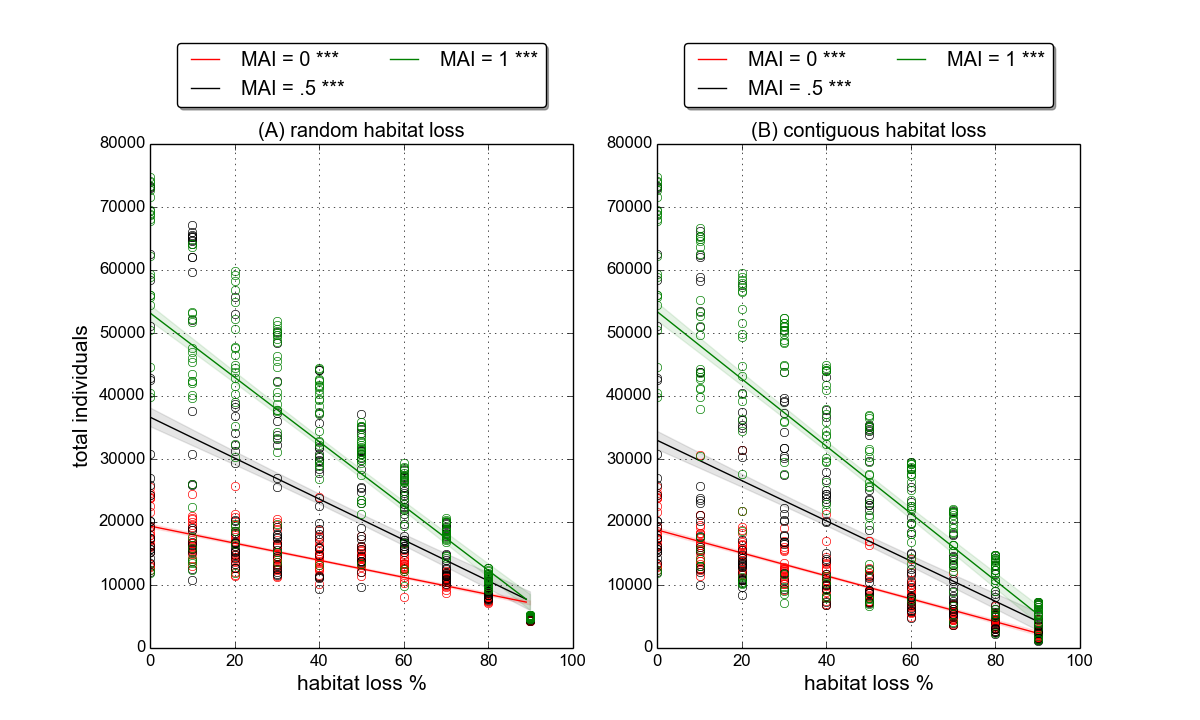
\includegraphics[width=\textwidth]{{{clean_figs/clean_lm_total_count_3mai}}}
	\caption{\textbf{Total number of individuals} against percentage habitat loss, for both scenarios: (A) Random HL, and (B) Contiguous HL. Circles represent the number of individuals for a single community; lines represent a linear fit to the data and the shaded regions indicate the standard error of the mean. \emph{p}-value $<0.001$ for all linear model fits (indicated by ***).}
	\label{fig:total_individuals}
	% This fig and shannon_eq created with: linear_models/ecosystem/clean_lm_general.py
\end{figure}

\begin{figure}
	\centering
	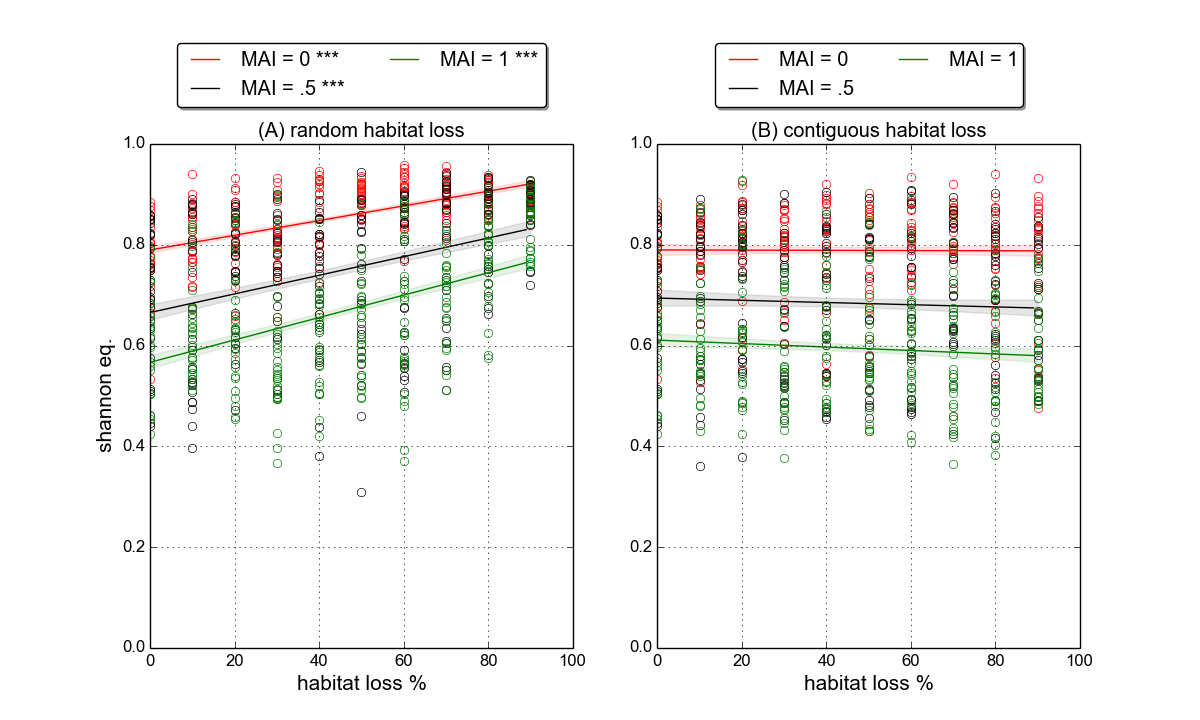
\includegraphics[width=\textwidth]{{{clean_figs/clean_lm_shannon_eq_3mai}}}
	\caption{\textbf{Shannon diversity} against percentage habitat loss, for both scenarios: (A) Random HL, and (B) Contiguous HL. Circles represent the Shannon index value for a single community; lines represent a linear fit to the data and the shaded regions indicate the standard error of the mean. *** indicates p-value $<0.001$ for linear model fit, whilst no marker indicates p-value$>0.1$.}
	\label{fig:shannon_eq}
\end{figure}


Figure \ref{fig:total_individuals} shows that the total number of individuals decreases in response to HL, in both the random and contiguous scenarios. This is expected - as the number of available cells becomes fewer the landscape is able to support fewer individuals. The linear fits to the data suggest that the average number of individuals is the similar at each point in the HL gradient in the two HL scenarios. Therefore there is little to distinguish between the scenarios based on the number of individuals. The figure also shows that communities with higher MAI ratio support more individuals than those with lower MAI ratio, as previously reported \cite{lurgi2015effects}.

%The main difference between the scenarios is at $90\%$ HL where there is visibly more variability between replicates in the contiguous case than the random\footnote{Either remove this statemetn or refer back to it later..}. 

Despite the decreases in the total number of individuals species do not go extinct (results not shown). At $90\%$ HL, when averaged over all AMI ratios and replicates, we observed a mean of $0.0$ and $0.23$ species extinctions per community for random and contiguous HL respectively. Therefore we effectively see \emph{no change in species richness} in response to habitat loss. The lack of extinctions is due to a relatively high immigration rate (IR). The default value of IR$=0.005$ means that, if the landscape were empty, we expect  on each time step an average of 200 ($=0.005 \times 200 \times 200$) immigrant individuals draw uniformly at random from the pool of 600 species. Therefore species may recover from extinction via a \emph{rescue effect} that is common to all species. The immigration mechanism also allows for the maintenance of very low species abundances, which are maintained by immigration rather than interactions. The absence of extinctions is an interesting feature of these results, since it allows us to focus on underlying structural changes that are not associated with the loss of species (see section \ref{sec:intro_habitat_loss} for literature relating to this issue, and section \ref{sec:discussion} for discussion relating to these results).

Although we do not observe changes in species richness under either HL scenario, we do see changes in community structure. Figure \ref{fig:shannon_eq} shows that the normalised \emph{Shannon diversity} (equation \ref{eq:shannon_eq}) increases for random HL, but does not change significantly for contiguous HL. The same trends are observed when diversity is calculated for each functional group separately (results not shown). This tells us that communities, both at the community level and within functional groups, become more diverse under random HL, whereas under contiguous HL there are \emph{no significant changes in diversity}. Since we know that there is no change in the number of species, any change in diversity must be driven by changes in \emph{evenness} in the distribution of species abundances.
 
\begin{figure}[hb]
	\centering
	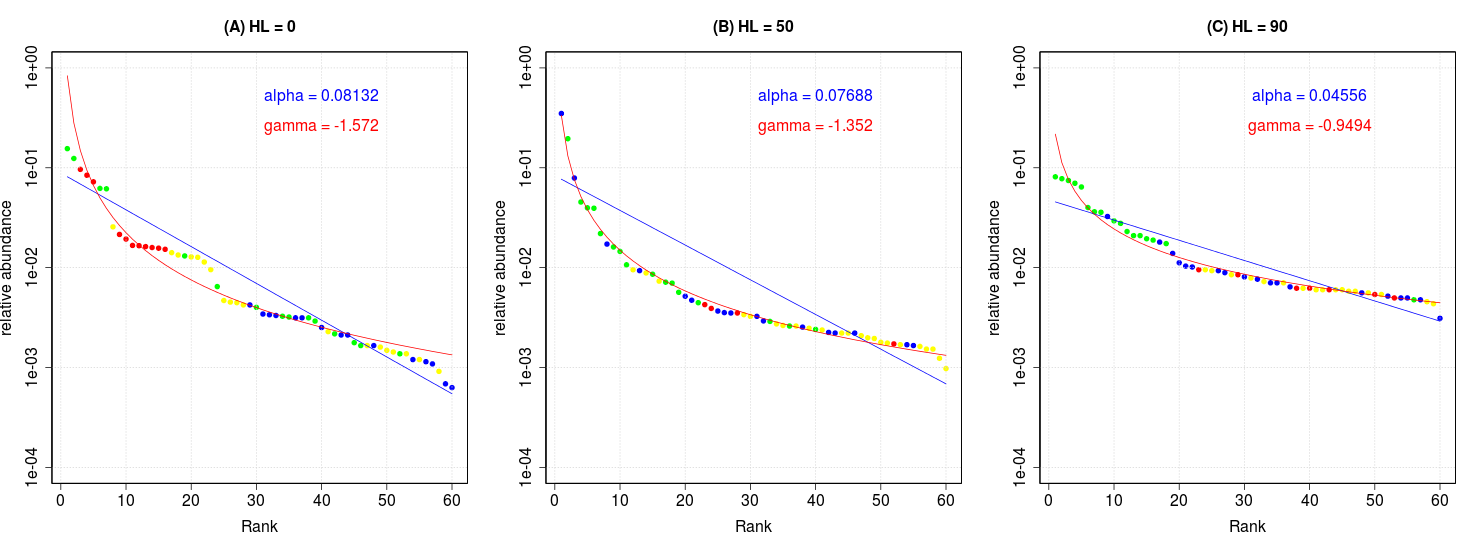
\includegraphics[width=\textwidth]{{{clean_figs/rad_3examples_random_mai0.5}}}
	\caption{\textbf{Example rank abundance distributions (RADs)} for three communities with \textbf{MAI=0.5} at different levels of \textbf{random HL}: (A) HL$=0\%$; (B) HL$=40\%$; (C) $80\%$. Species abundances are relative to the total number of individuals in the community, and plotted on a logarithmic scale. Points represent species, coloured according to trophic level: green=basal; blue=herbivore/animal-mutualist; yellow=omnivore; red=top predator. Colours consistent with other figures that show trophic information. Blue and red lines give the pre-emption and Zipf model fits respectively (see text in section \ref{sec:define_rads} for definitions), best fit parameter value for each model given as annotations on plot.}
	\label{fig:example_rads_random}
	%% This an other example rad created with r-script: RADs_neat_fit.r
\end{figure}

\begin{figure}[hb]
	\centering
	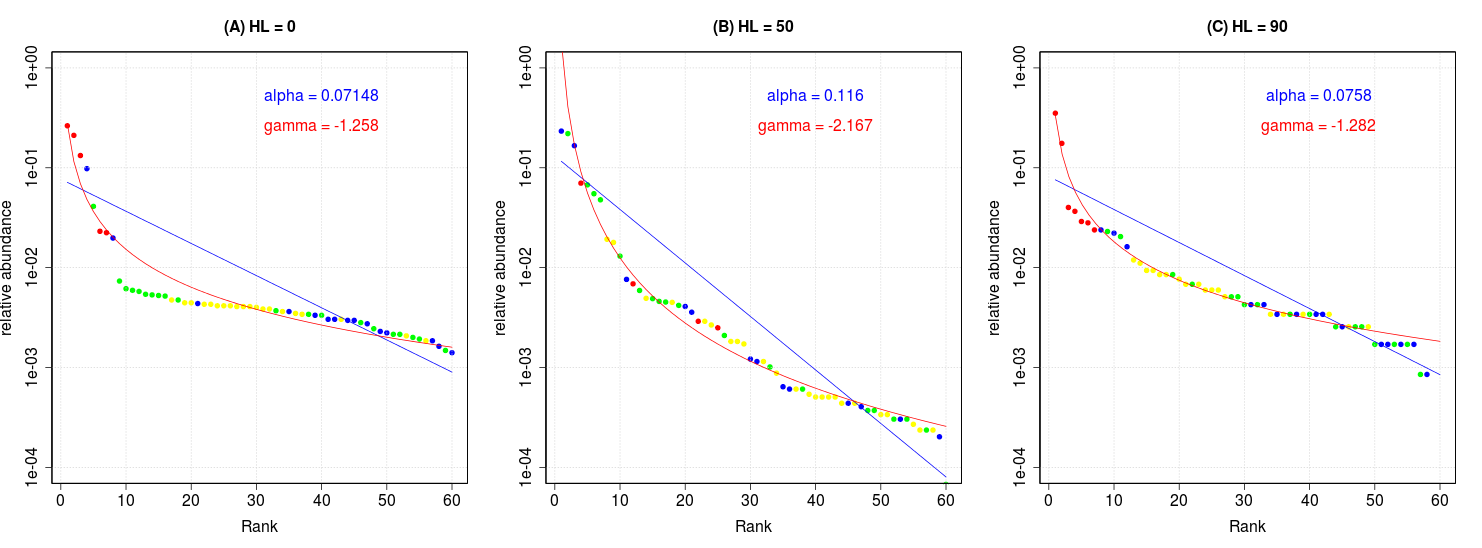
\includegraphics[width=\textwidth]{{{clean_figs/rad_3examples_contiguous_mai0.5}}}
	\caption{Similar to figure \ref{fig:example_rads_random} but for \textbf{contiguous HL}.}
	\label{fig:example_rads_contiguous}
\end{figure}
 
 
To look explicitly at changes in evenness we construct \emph{rank abundance distributions} (RADs) for each community, and fit standard models to these distributions (defined in section \ref{sec:define_rads}). Figures \ref{fig:example_rads_random} and \ref{fig:example_rads_contiguous} show example RADs for three communities at different levels of HL, all with MAI$=0.5$. Since these plots are for single communities we cannot draw general conclusions from them. However, they serve to visualise the model fits and their interpretation. The solid blue and red lines in these plots show the \emph{preemption} and \emph{Zipf} model fits to the RADs, respectively. Each model has an evenness parameter and, as discussed in section \ref{sec:define_rads}, the lower the magnitude of the parameter the more even the distribution. From visual inspection panel C in figure \ref{fig:example_rads_random} is the most even RAD of the six displayed. Correspondingly the model fits to this RADs have the lowest magnitude values for $\alpha$ and $\gamma$. Although the Zipf model appears to give a qualitatively better fits to the data, we use both models the test for evenness in our simulated communities. In this way we can check for consistency in the conclusions.


\begin{figure}
	\centering
	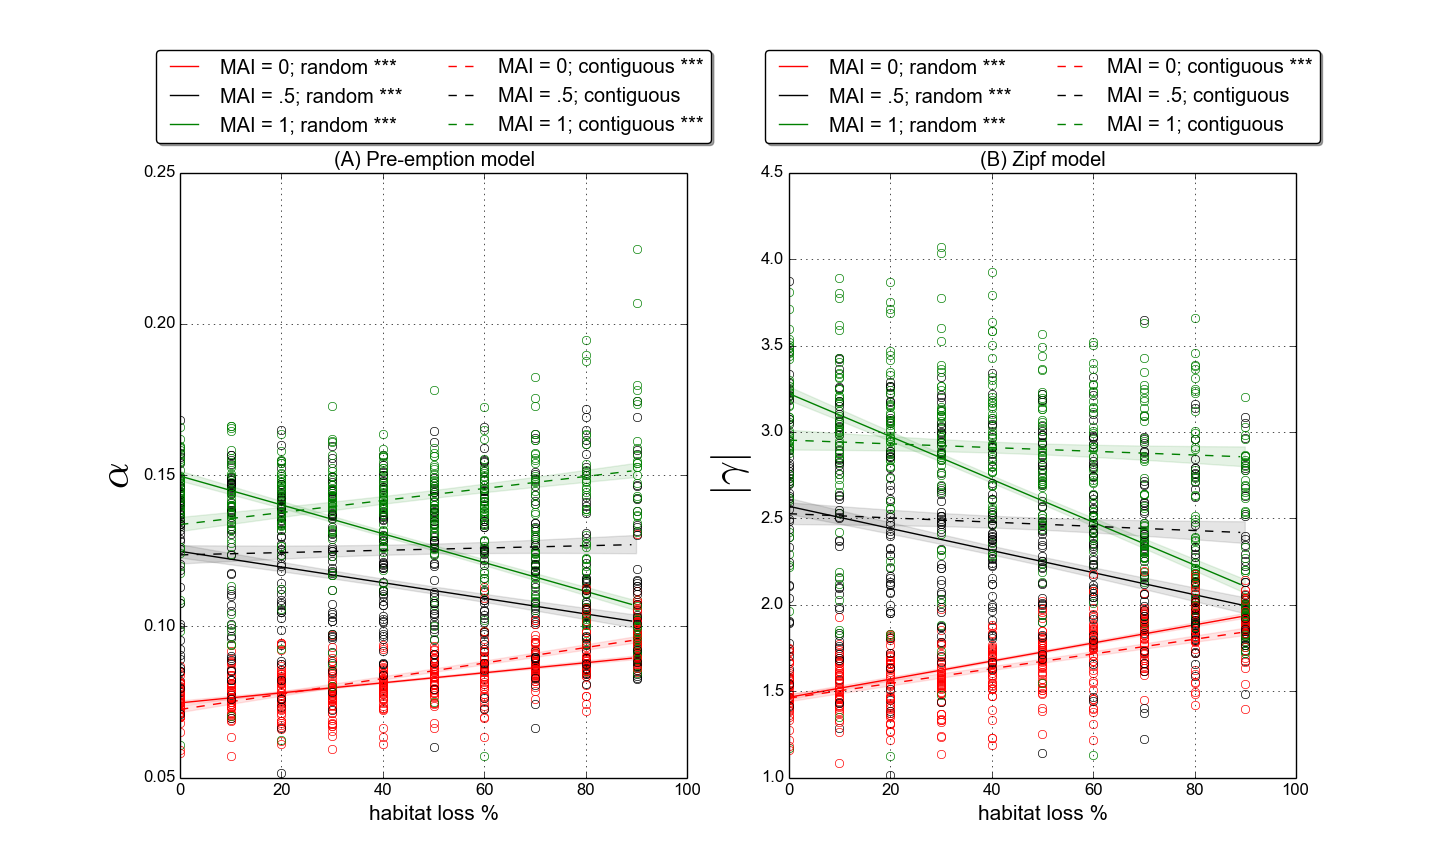
\includegraphics[width=\textwidth]{{{clean_figs/lm_radfit_params_v_hl}}}
	\caption{\textbf{Rank abundance model fit} parameters against HL. Panel A: Pre-emption model parameter $\alpha$ is smaller for more even distributions. Panel B: Absolute value of Zipf model parameter $\left| \gamma \right|$ is smaller for more even distributions. (See model definitions in section \ref{sec:define_rads}). Solid lines represent linear fits to the random HL data, dashed lines indicate linear fits to the contiguous HL data, and error bars give $\pm 1$ standard-deviation. *** indicates p-value $<0.001$ for linear model fit, whilst no marker indicates p-value$>0.1$.}
	\label{fig:radfit_params}
	% Results compiled with radfit_param_v_hl.r
	% Plotted with lm_rad_v_hl.py (bespoke!)
\end{figure}


Figure \ref{fig:radfit_params} shows how the evenness parameters, $\alpha$ and $\gamma$, change in response to HL. For clarity the results are shown for two MAI ratios only ($0.0,1.0$), but are consistent across all MAI ratios. The modelling suggests that under contiguous HL the RADS shown no significant change in evenness. However both the preemption and Zipf models indicate that communities under random HL show a significant increase in evenness. These findings are consistent with the changes in Shannon diversity discussed above. 

The RADs in figure \ref{fig:example_rads_random} suggest another trend in response to random HL - there appears to be a systematic shift in the relative abundances according to trophic level. This is most visible for the basal and top trophic levels, shown in green and red respectively. For the example communities shown, the top predator species have high relative abundance in pristine landscape (HL$=0$), but reduced abundances after habitat loss. At $90\%$ HL all top predators in the community shown have a relative abundance less than 0.01. On the other hand basal species have a wide range of relative abundances in pristine landscape, but come to dominate the community at $90\%$ HL with all but one basal species in the top 18 ranks. To investigate this effect further we look at the relative abundances of all six functional groups in response to habitat loss.  These are plotted in figures \ref{fig:rel_abun_random} and \ref{fig:rel_abun_contiguous} for the random and contiguous scenarios respectively. For the contiguous scenario community structure, according to these relative abundances, is remarkably constant across the habitat loss gradient. The only statistically significant changes are in the non-mutualistic plant and top predator species at MAI$=0$, where there is a slight decrease in top predator abundance relative to plant abundance. In the random scenario there are clear systematic shifts in the distribution of abundance across functional groups. In particular there is a relative increase in plant abundance and decrease in top predator abundance, which is statistically significant across all MAI ratios. There is also a slight decrease in the relative abundance of species in the second trophic level (herbivores and mutualistic animals). Overall there is a shift in relative abundance towards the basal level, but interestingly there is no significant change in the abundance of omnivore species. This suggests that there is some benefit to being omnivorous in this context (see discussion in \ref{sec:res_synthesis}).  


\begin{figure}[p]
	\centering
	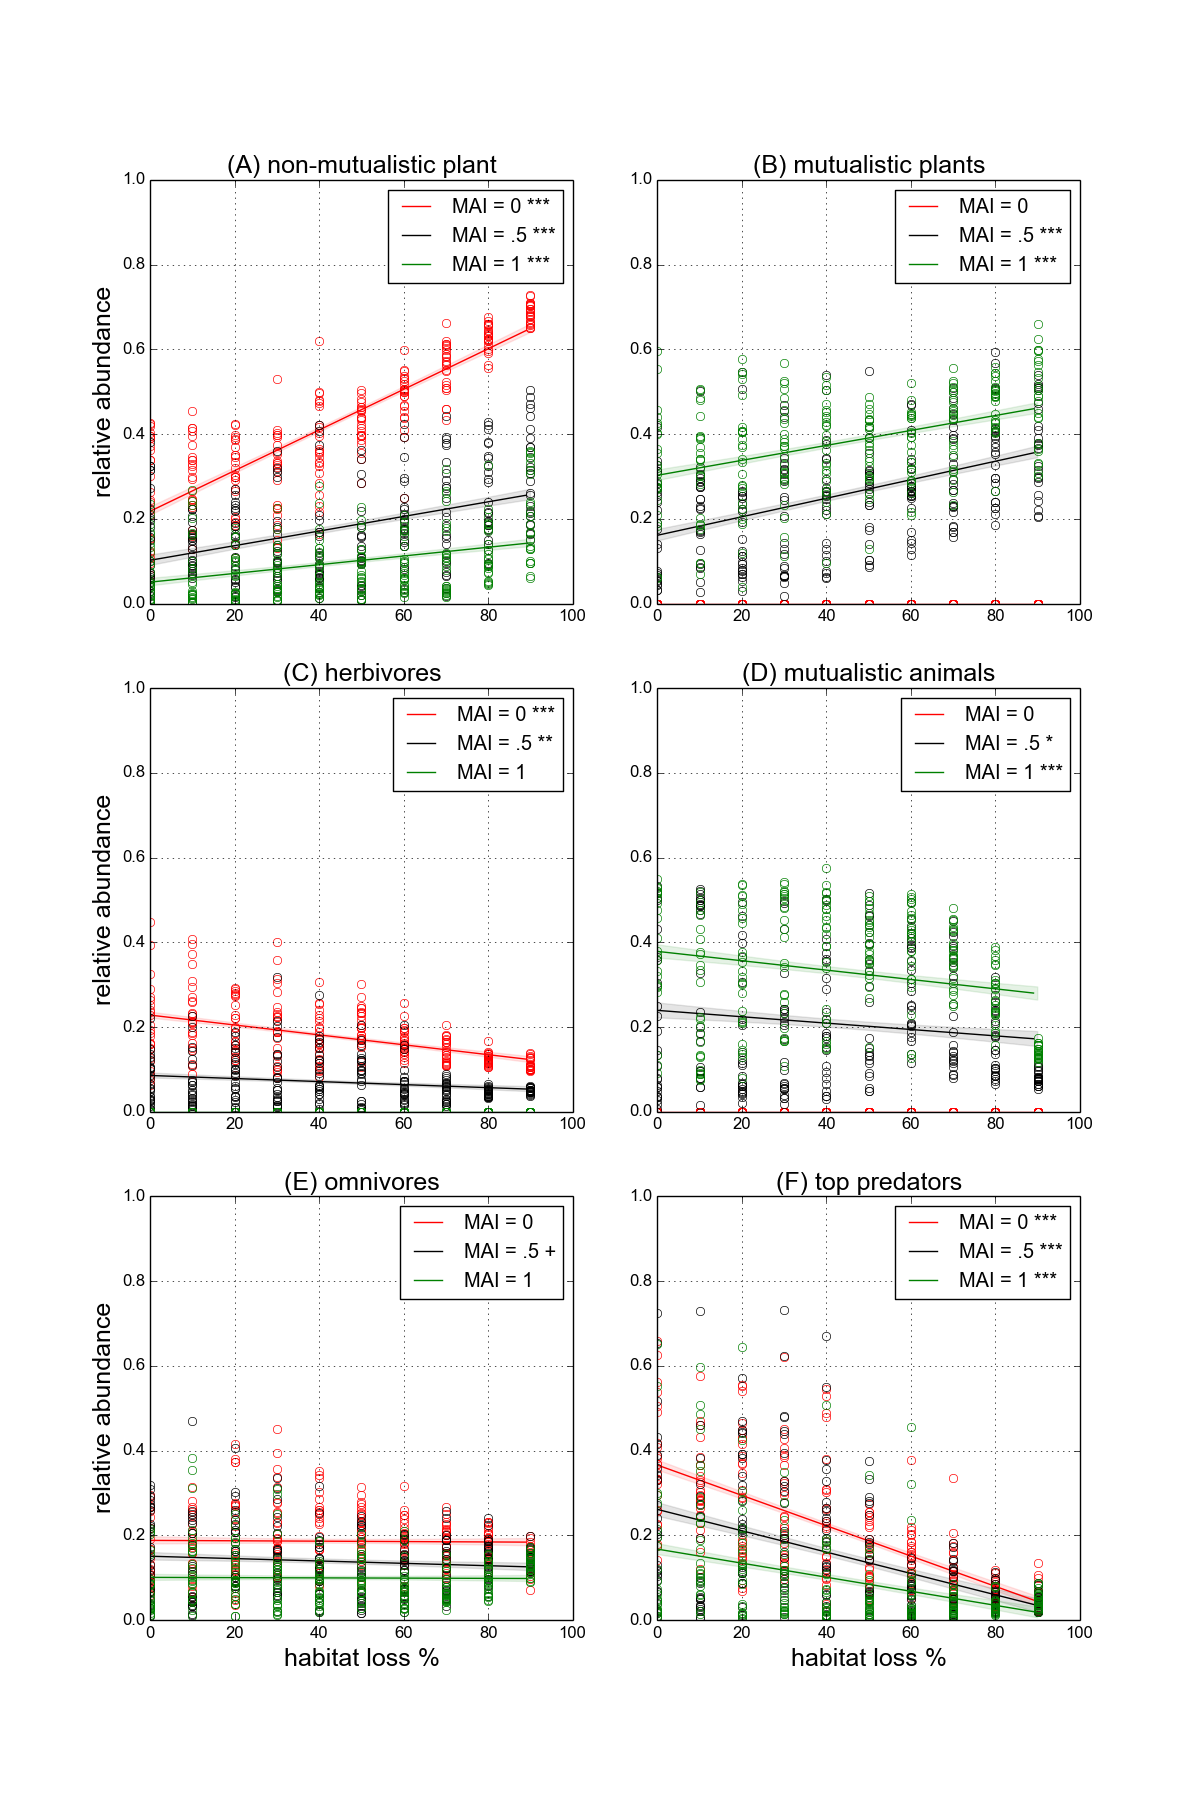
\includegraphics[width=0.8\textwidth]{{{clean_figs/lm_fg_relative_abundance_hl_random_3mai}}}
	\caption{\textbf{Relative abundance} by functional group for \textbf{random HL}. Abundance relative to total number of individuals in the community. Circles represent the value for a single community; lines represent a linear fit to the data and the shaded regions indicate the standard error of the mean. The markers ***, **, * and + corresponds to linear model fit p-values of $<0.001$, $<0.01$, $<0.05$ and $<0.1$ (marginal significance) respectively.}
	\label{fig:rel_abun_random}
\end{figure}

\begin{figure}[p]
	\centering
	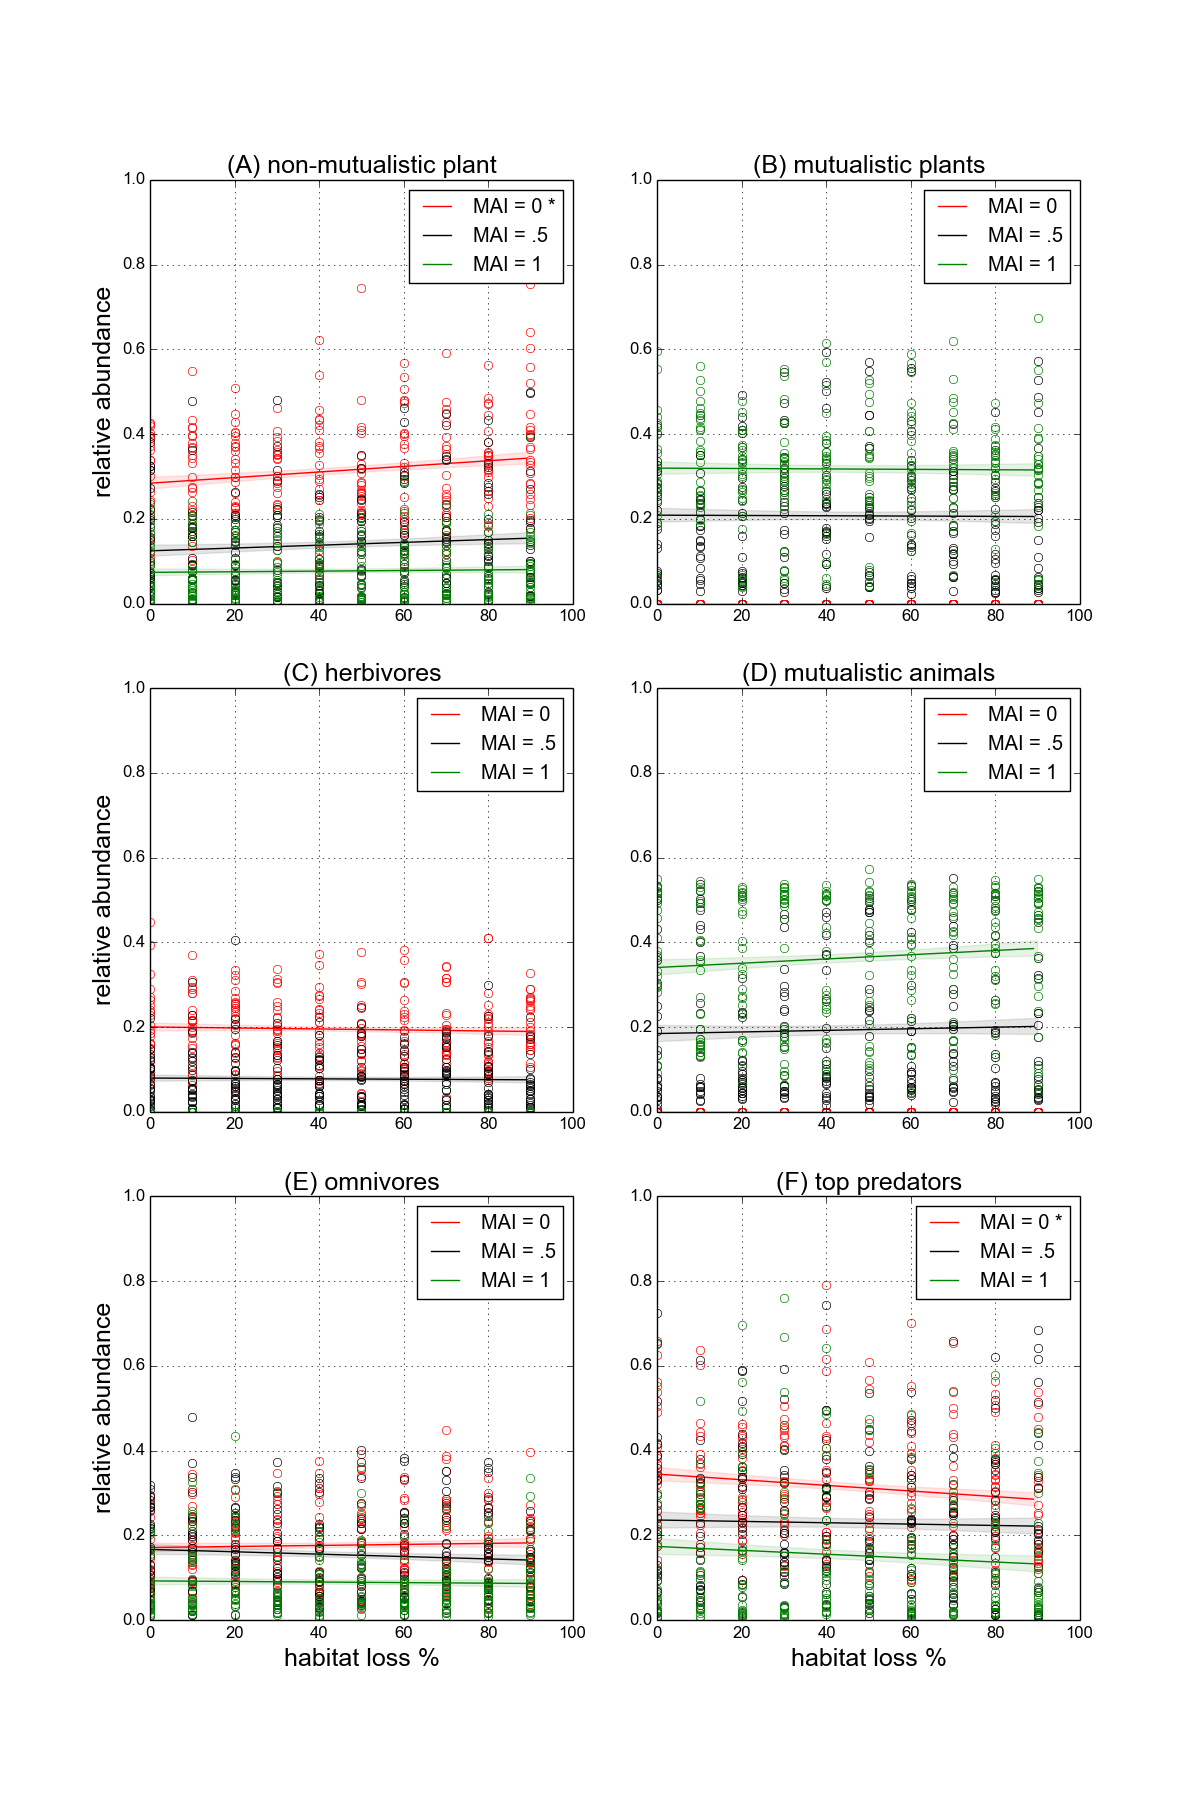
\includegraphics[width=0.8\textwidth]{{{clean_figs/lm_fg_relative_abundance_hl_contiguous_3mai}}}
	\caption{Similar to figure \ref{fig:rel_abun_random}, but for \textbf{contiguous HL}.}
	\label{fig:rel_abun_contiguous}
\end{figure}

\clearpage
\subsection{Network properties}
\label{sec:res_network_properties}

Figure \ref{fig:num_links} shows that, in both HL scenarios, there is a slight decrease in the number of links in the realised network. This result indicates that some species, which would be able to interact, do not encounter each other in space as a result of HL. The number of links lost, on average is few - the greatest loss according to the linear models is under contiguous HL for MAI$=1.0$ where the number of links falls from $\approx 250$ in pristine landscape to $\approx 200$ at $HL=90\%$\footnote{Why is the greatest change here?}. However loosing any number of links may be enough to create detectable changes in network topology. In addition to the loss of links from the network we see a decrease in the total number of interactions in both scenarios, which is shown in figure \ref{fig:total_interactions}. This is in agreement with the loss of individuals (figure \ref{fig:total_individuals}), since if there are fewer individuals in the landscape we should expect fewer interactions. In general we expect the frequency on an interaction to be largely determined by the abundances of the interacting species. This effect was discussed in section \ref{sec:WHEREIS}, and is studied in more detail in chapter \ref{chap:inferring_interactions}. However it appears from figure \ref{fig:total_interactions} that more interactions are lost due to random HL than contiguous, since the slopes of the linear fits are steeper\footnote{Also look at high HL values - it is clear.}. This suggests a mechanism under random HL that results in fewer interactions than under contiguous HL, despite similar numbers of individuals. We propose such a mechanism in section \ref{sec:res_synthesis}.  


%Interactions driven by abundances! See chapter \ref{chap:inferring_interactions} for more on this. Need to plot here?

\begin{figure}
	\centering
	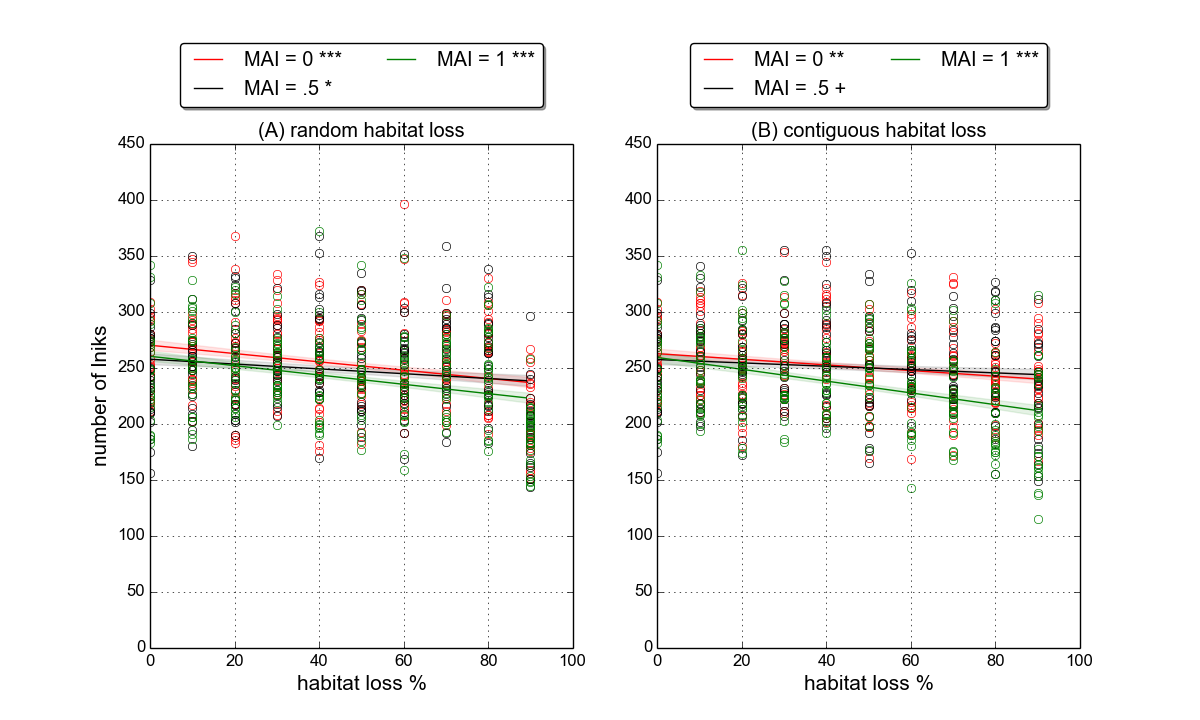
\includegraphics[width=0.8\textwidth]{{{clean_figs/clean_lm_number_of_links_3mai}}}
	\caption{\textbf{Number of links} of links in the realised network (see text in section \ref{sec:sampling} for definition). Linear fits and p-value markers as in previous plots (see caption of figure \ref{fig:rel_abun_random}).}
	\label{fig:num_links}
\end{figure}

\begin{figure}
	\centering
	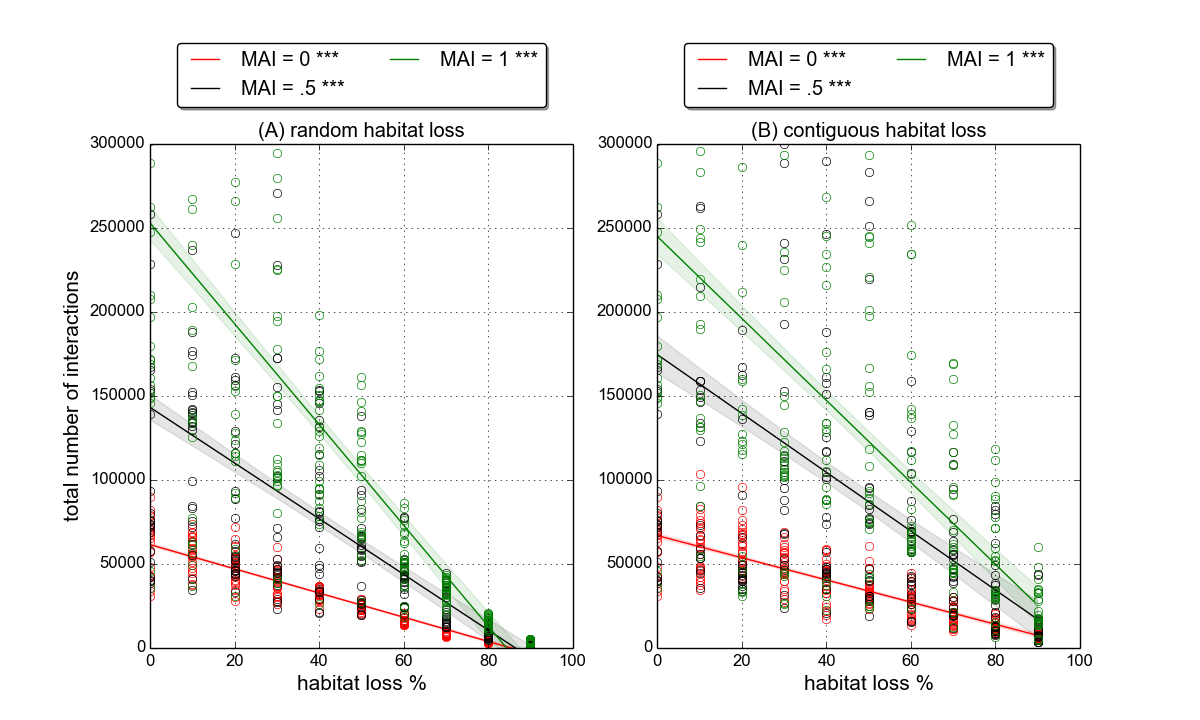
\includegraphics[width=0.8\textwidth]{{{clean_figs/clean_lm_total_interactions_3mai}}}
	\caption{\textbf{Total number of interactions} between all species during final 200 iterations of a simulation. Linear fits and p-value markers as in previous plots (see caption of figure \ref{fig:rel_abun_random}).}
	\label{fig:total_interactions}
\end{figure}

Together the loss of links, and the change in interaction frequencies indicate changes in realised network of interactions. Therefore we to seek to characterise these changes, using the network metrics defined in section \ref{sec:define_network_metrics}. The nestedness and compartmentalisation of communities showed no significant change under either HL scenario. Therefore these plots are not shown. The response of the binary metrics follows directly from the loss of links, since there is no change in species richness. Therefore connectance, generality and vulnerability all decrease in both scenarios (results not shown), as a result of the loss of links shown in figure \ref{fig:num_links}. The response of the quantitative network metrics is more interesting because these metrics are based not only on the presence/absence of links, but on the frequency of each interaction. 

The results for the weighted quantitative generality and vulnerability metrics (hereafter generality and vulnerability) are shown in figures \ref{fig:generality} and \ref{fig:vulnerability}. For contiguous HL neither metric shows significant change. This tells us that the loss of links and decrease in interaction frequencies occur in a such a way that the average number of effective prey and predators per species is constant across the contiguous HL gradient. For this to occur the changes must be distributed homogeneously across the network such that there is no change, on average, in the number of interactions per species and the relative frequencies of those interactions. This finding is in agreement with the observed lack of change in diversity and abundance patterns under contiguous HL (section \ref{sec:res_diversity}) - if the relative abundance of all species is constant across the HL gradient, and interaction frequencies are mainly driven by species abundances, then the lack of change in quantitative network metrics follows directly. This appears to be what is happening in the contiguous scenario\footnote{I understand this but maybe it is not clear?}.

In the random scenario quantitative generality and vulnerability decrease and increase respectively (figures \ref{fig:generality} and \ref{fig:vulnerability}). This represents ad asymmetry between the responses of predator interactions compared to prey interactions. The increase in vulnerability means that the average \emph{effective} number of predators per prey increases. It is unlikely that the \emph{actual} number of predators per prey increases, since links are lost form the network. Therefore the only way that vulnerability could increase is if the interaction frequencies of prey with their predators become more even. We know from section \ref{sec:res_diversity} that species abundances become more even in response to random HL, and that diversity increases both at the community level and within functional groups. Therefore the change in vulnerability appears to be explained by changes in species abundances.  

The drop in generality tells us that the average \emph{effective} number of prey per predator decreases under random HL. Since we have just concluded that interaction frequencies become more even, we must attribute this to a decrease in the \emph{actual number of prey} per predator. Since we know that the relative abundance of top predators is greatly reduced (figure \ref{fig:rel_abun_random}), it is reasonable to conclude that some struggle to find prey. Interestingly the change in generality at MAI$=1.0$ is not significant (although it was significant at all other MAI ratios) suggesting that either prey are not lost, or more likely that the loss of prey to top predators is offset by the increased evenness of interactions. We know that high MAI communities have fewer top predators and so their contribution to generality is likely to be less. Also high MAI communities contain more individuals than low MAI communities across the HL gradient, meaning a greater absolute number of prey. Together these two mechanisms may be enough to explain why generality does not change at MAI$=1.0$.   

%Our explanation of the change in generality suggests that the average \emph{actual} number of predators per prey to decreases. 

\begin{figure}
	\centering
	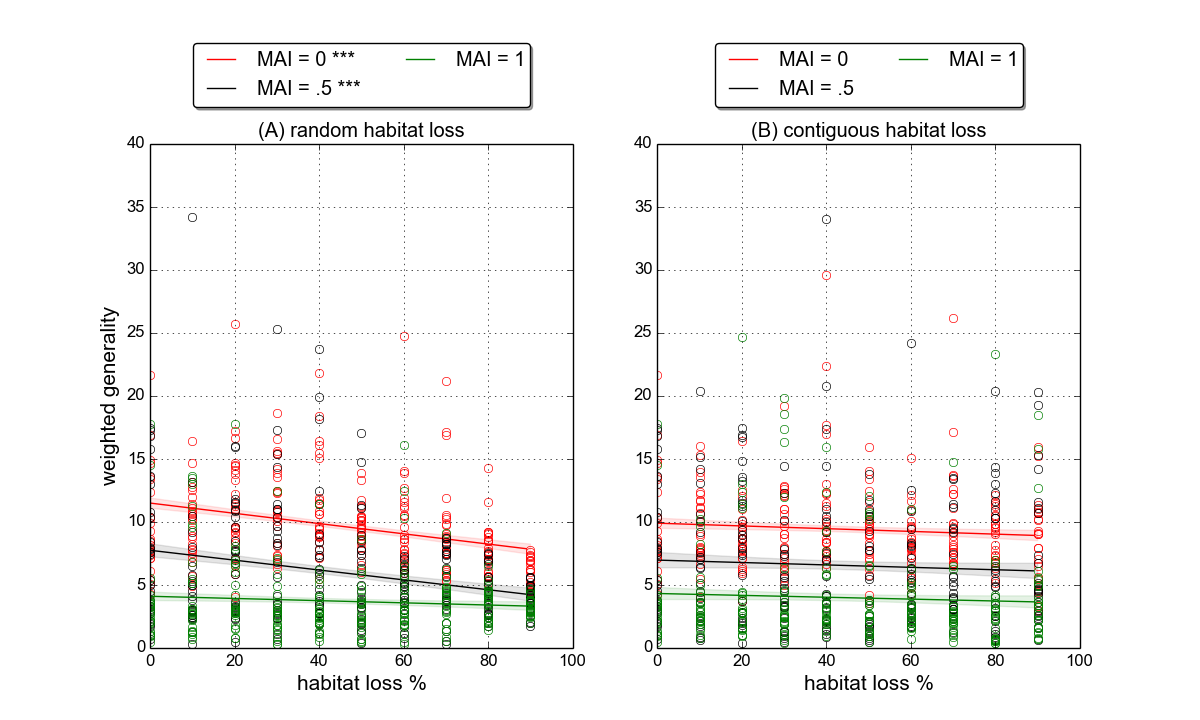
\includegraphics[width=0.8\textwidth]{{{clean_figs/clean_lm_weighted_generality_3mai}}}
	\caption{\textbf{Weighted quantitative generality}, of whole network (see section \ref{sec:define_network_metrics} for definition). Linear fits and p-value markers as in previous plots (see caption of figure \ref{fig:rel_abun_random}).}
	\label{fig:generality}
\end{figure}

\begin{figure}
	\centering
	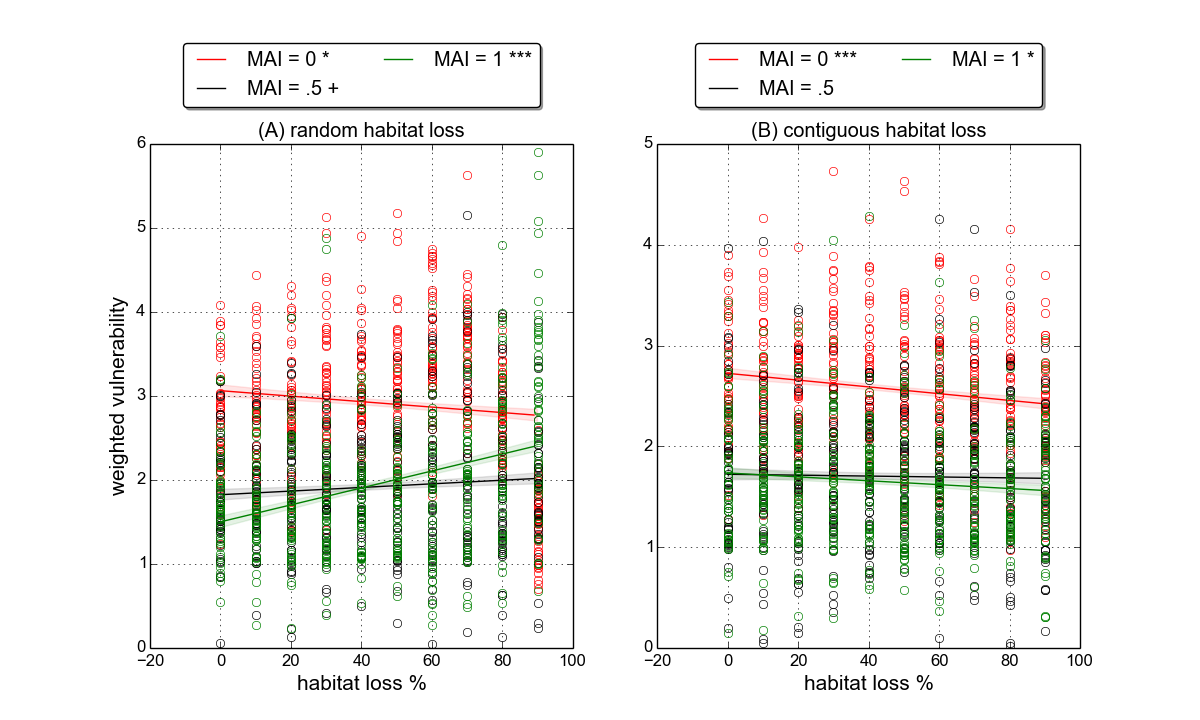
\includegraphics[width=0.8\textwidth]{{{clean_figs/clean_lm_weighted_vulnerability_3mai}}}
	\caption{\textbf{Weighted quantitative vulnerability}, of the whole network (see section \ref{sec:define_network_metrics} for definition). Linear fits and p-value markers as in previous plots (see caption of figure \ref{fig:rel_abun_random}).}
	\label{fig:vulnerability}
\end{figure}

The results for the bipartite network metrics, interaction diversity and H2', are shown in figures \ref{fig:interaction_diversity} and \ref{fig:specialisation}. They support the conclusion that the changes in quantitative network metrics are driven by changes in species relative abundances. In the contiguous scenario neither metric shows significant changes, in agreement with the generality and vulnerability results. In the random scenario interaction diversity increases, whereas the specialisation metric H2' shows no significant change. The increase in interaction diversity is in agreement with the proposed increase in evenness of interaction frequencies due to increased evenness in species abundances. The lack of change in H2' means that interactions, in the mutualistic sub-network, do not become more even than expected based on the constraints imposed on $H2_{min}$ and $H2_{max}$ (see definitions in section \ref{sec:define_network_metrics}). The implementation of H2' that we used has the constraint that the total number of interactions of each species is held constant. It is reasonable to assume, as discussed, that the total number of interaction of a species is proportional to its abundance. Therefore we may interpret the lack of a trend in H2' as saying that interactions do not become more even than expected, given the abundance of each species. In other words, the change in the diversity of interactions is due to changes in species relative abundances, as we expected.

\begin{figure}
	\centering
	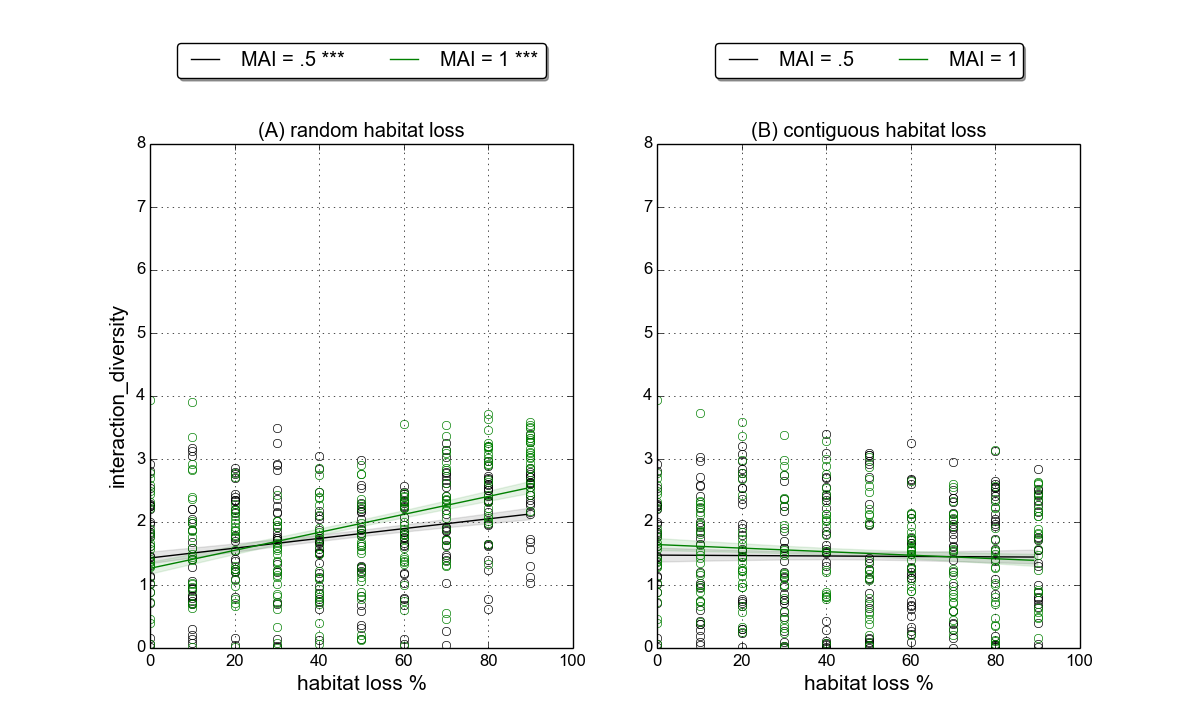
\includegraphics[width=0.8\textwidth]{{{clean_figs/clean_lm_interaction_diversity_3mai}}}
	\caption{\textbf{Interaction diversity} in the mutualistic sub-network (see section \ref{sec:define_network_metrics} for definition). Linear fits and p-value markers as in previous plots (see caption of figure \ref{fig:rel_abun_random}).} 
	\label{fig:interaction_diversity}
\end{figure}

%\begin{figure}
%	\centering
%	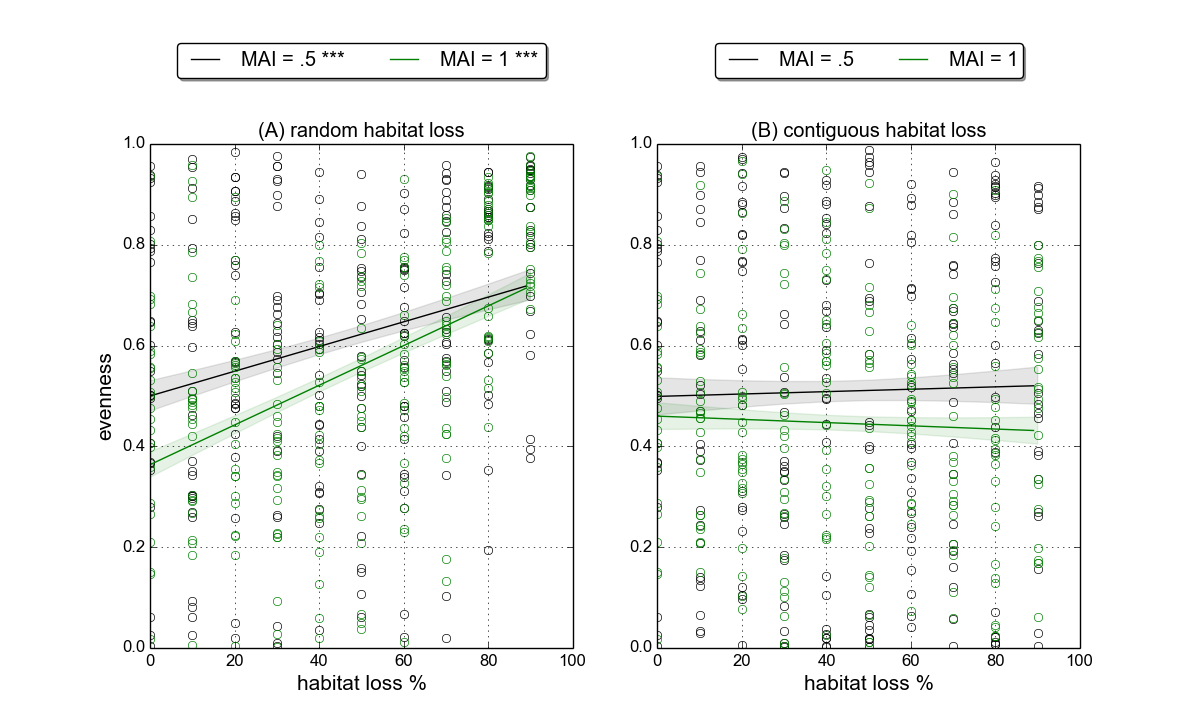
\includegraphics[width=0.8\textwidth]{{{clean_figs/clean_lm_evenness_3mai}}}
%	\caption{\textbf{Interaction evenness} in the mutualistic sub-network.}
%	\label{fig:interaction_evenness}
%\end{figure}

\begin{figure}
	\centering
	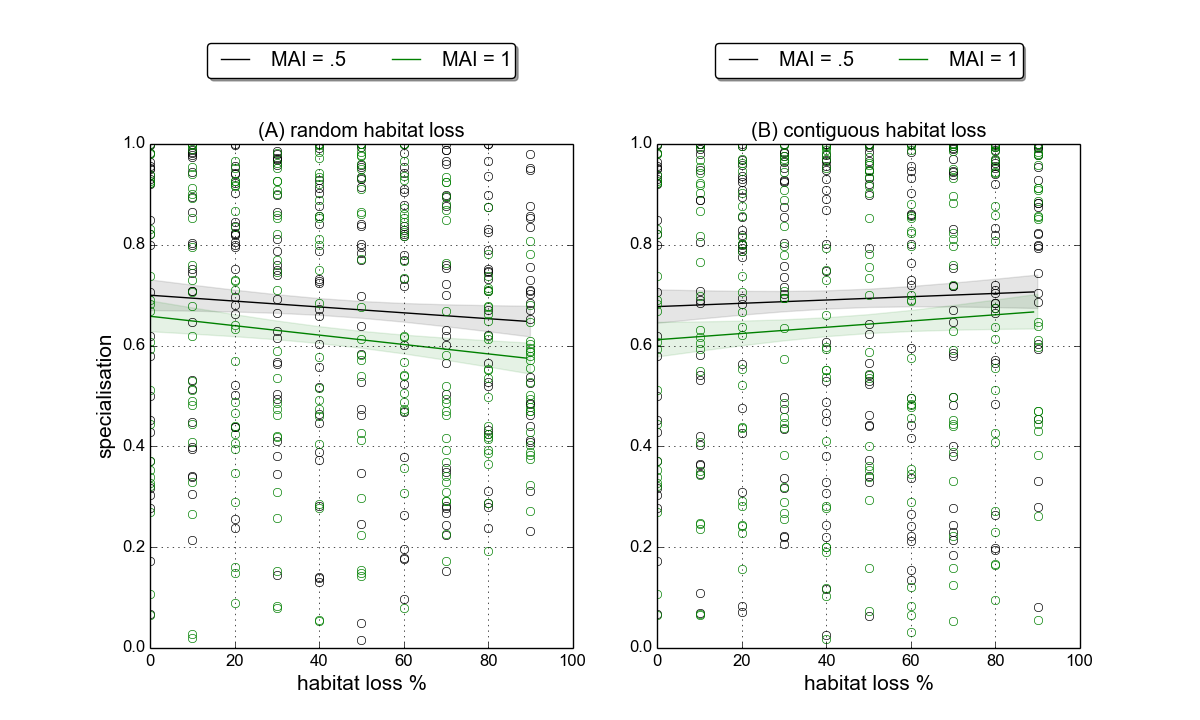
\includegraphics[width=0.8\textwidth]{{{clean_figs/clean_lm_specialisation_3mai}}}
	\caption{\textbf{Specialisation H2'} in the mutualistic sub-network (see section \ref{sec:define_network_metrics} for definition). Linear fits and p-value markers as in previous plots (see caption of figure \ref{fig:rel_abun_random}).}
	\label{fig:specialisation}
\end{figure}


\clearpage
\subsection{Stability and Space}
\label{sec:res_stability_and_space} 

\begin{figure}[b]
	\centering
	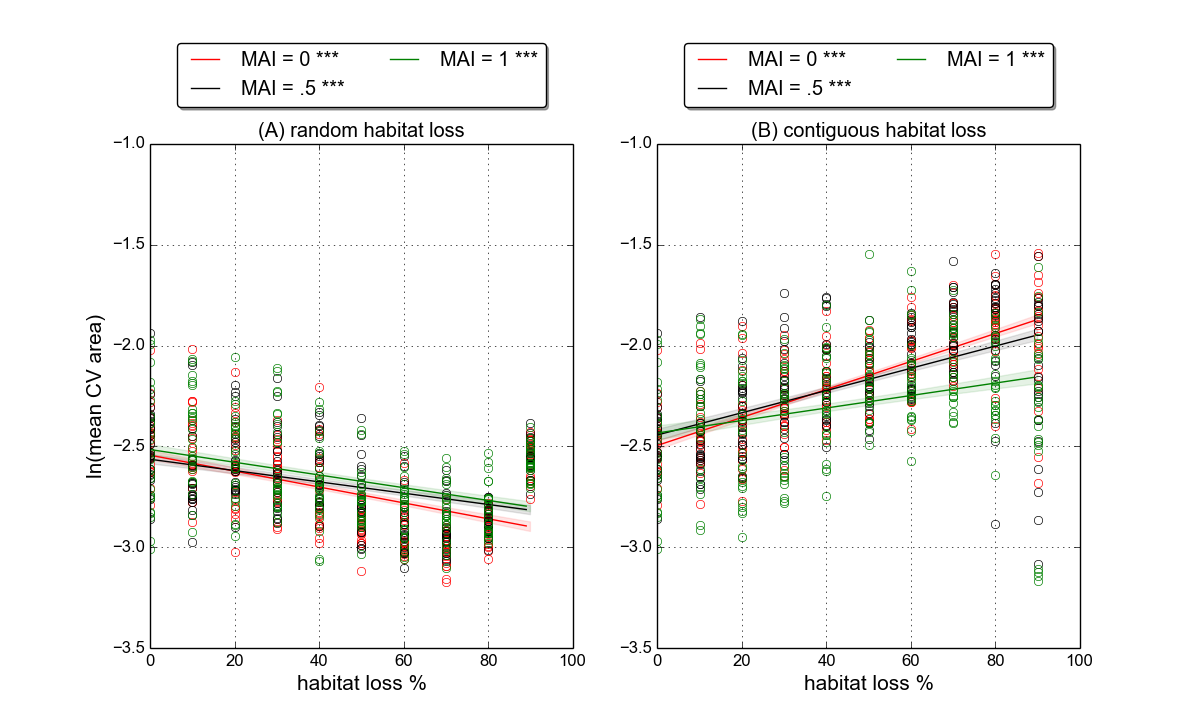
\includegraphics[width=0.9\textwidth]{{{clean_figs/clean_lm_mean_cv_area_3mai}}}
	\caption{\textbf{Species area variability}: coefficient of variation in area of species range, averaged over all species (definition in section \ref{sec:def_stability_metrics}). Linear fits and p-value markers as in previous plots (see caption of figure \ref{fig:rel_abun_random}).}
	\label{fig:mean_cv_area}
\end{figure}

\begin{figure}
	\centering
	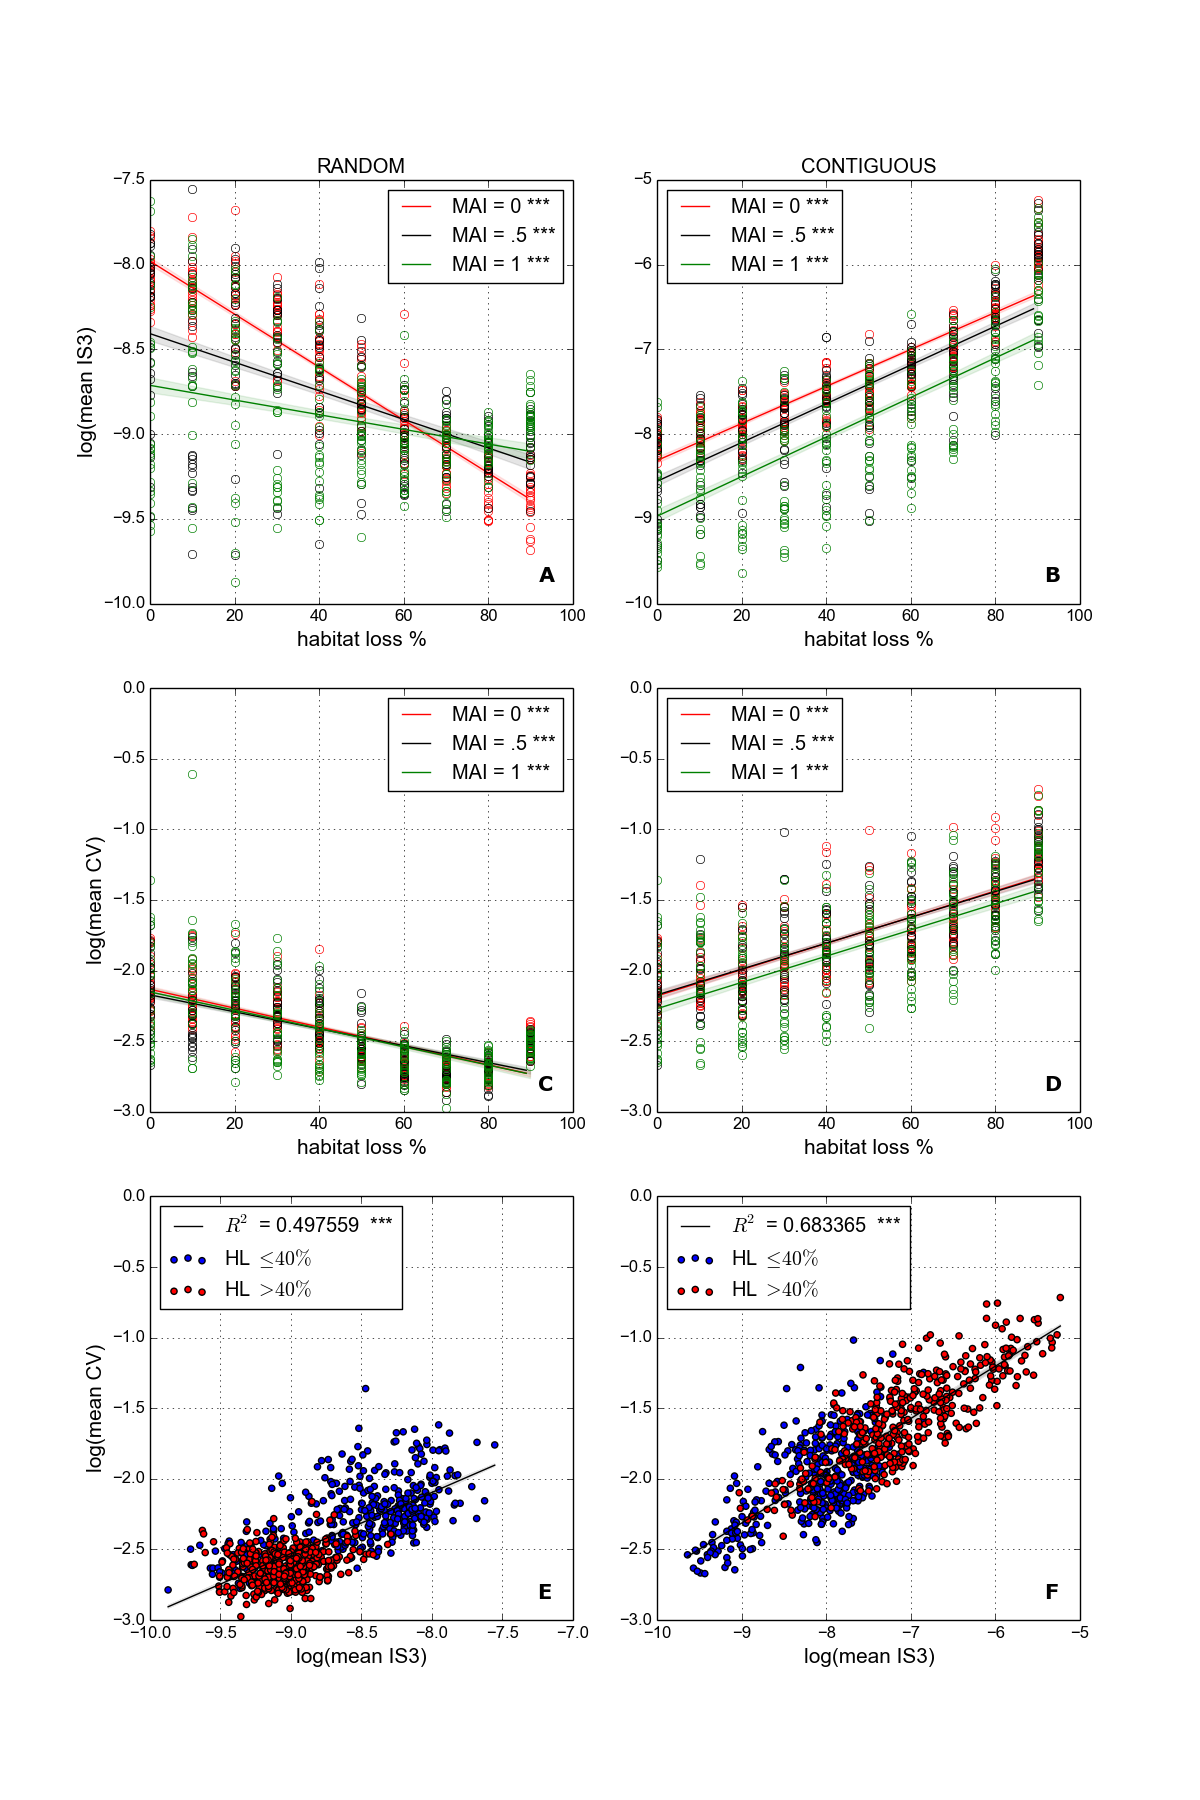
\includegraphics[width=0.8\textwidth]{{{clean_figs/strong_fig}}}
	\caption{\textbf{Interaction strengths and temporal variability.} Both natural log-transformed to linearise trends. Panels A-B: Interaction strength metric IS3 (defined in section \ref{sec:def_stability_metrics}) averaged over all interactions in realised network. Panels C-D: mean CV, coefficient of variation in species abundances (defined in section \ref{sec:def_stability_metrics}) averaged over all species. Panels E-F: IS3 as a linear predictor for mean CV, with low and high HL communities indicated by blue and red circle respectively. Linear fits and p-value markers as in previous plots (see caption of figure \ref{fig:rel_abun_random}).}
	\label{fig:strong_fig}
\end{figure}

%As discussed in section \ref{sec:stability} there are several alternative stability metrics that can be calculated from population dynamics data. In this section we use the conventional metrics which are based on the coefficient of \emph{temporal variability}. In the following section (\ref{sec:res_invariability}) we demonstrate that the results for the metrics are consistent with the alternative stability metrics , which are based on \emph{invariability}.

In this section we measure stability using the four variability metrics defined in section \ref{sec:def_stability_metrics}: the temporal coefficients of variation (CV) in species abundances (\emph{mean CV}), species range area (\emph{mean CV area}), species range centroid (\emph{mean CV centroid}), and species spatial density (\emph{mean CV density}). At the end of the section we also look at the spatial aggregation metrics, as defined in section \ref{sec:def_stability_metrics}. Although these are not directly related to stability, they are relevant to the spatial structure of the communities. All metrics are calculated at the species level, and then averaged over all species in the community. In the following section (\ref{sec:res_invariability}) we show that the stability results are consistent with the alternative \emph{invariability} metrics, which are defined in section \ref{sec:stability}.

The stability results are consistent across the four variability metrics - \emph{communities become more variable under random HL, and less variable under contiguous HL}. To analyse the metrics we take the natural logarithm of the variability metrics before fitting linear models. The raw data show trends that are clearly non-linear, and appear approximately exponential (responses change at an increasing rate). Therefore the log-transform serves to linearise the data and make a linear model fit more appropriate. The log-linear trends are illustrated for species area variability in figure \ref{fig:mean_cv_area}, and for species abundance variability in the middle row of figure \ref{fig:strong_fig}. The same trends are observed for the other variability metrics (results not shown), and they are statistically significant across all MAI ratios. Therefore we conclude that the variability response is robust. The variability response also represents a striking difference between the two HL scenarios. In all other metrics presented communities either respond in the same way (e.g. number of individuals, number of links), or display significant changes under one scenario but not the other (for example evenness). However the trends observed in variability are qualitatively opposite for the two HL scenarios. This leads us to question the mechanism behind the change in variability.

The only metric, aside from variability, which shows trends in opposite directions under different types of HL is \emph{interaction strength} (IS3). These trends are illustrated in the top row of figure \ref{fig:strong_fig}, where we again use the natural log-transform of the data. Under random HL the average interaction strength decreases, whereas under contiguous HL it increases. We also observe the dependence of interaction strength on MAI ratio, as reported in \cite{lurgi2015effects}. In pristine landscape higher MAI communities have weaker interaction strengths. Under contiguous HL this ordering of IS3 according to MAI is conserved across the HL gradient. However under random habitat loss communities with a high MAI ratio do not lose interaction strength as much as low MAI communities. The result is that beyond about $70\%$ HL high MAI communities tend to have greater interaction strength that low MAI communities. Although only shown for three MAI ratios, the pattern described is consistent across all eleven MAI ratios. The possible explanations for the dependence of the IS3 response on MAI ratio are discussed in section \ref{sec:discussion}.

The bottom row (panels E and F) of figure \ref{fig:strong_fig} shows the log-transformed values of IS3 plotted against the log-transformed abundance variability. These figures are an aggregate representation of all the simulation repeats with MAI$=0.0,0.5,1.0$. In both the random and the contiguous scenario there is a significant linear trend between the log-transformed interaction strength and variability. The coefficient of determination $R^2$ values of these linear models are, as given on the plot, $\approx 0.5$ and $\approx 0.7$ in the random and contiguous cases respectively. This means that, on aggregate, interaction strengths can explain at least half of the variance in temporal variability, and more than this in the contiguous case\footnote{Also mention the red and blue points!}. We conclude that there is a strong correlation between IS3 and temporal variability in species abundances. In section \ref{sec:res_synthesis} we present the evidence that this correlation represents is a causal relationship, and that interaction strengths are key to understanding how simulated communities respond to HL.   

\begin{figure}
	\centering
	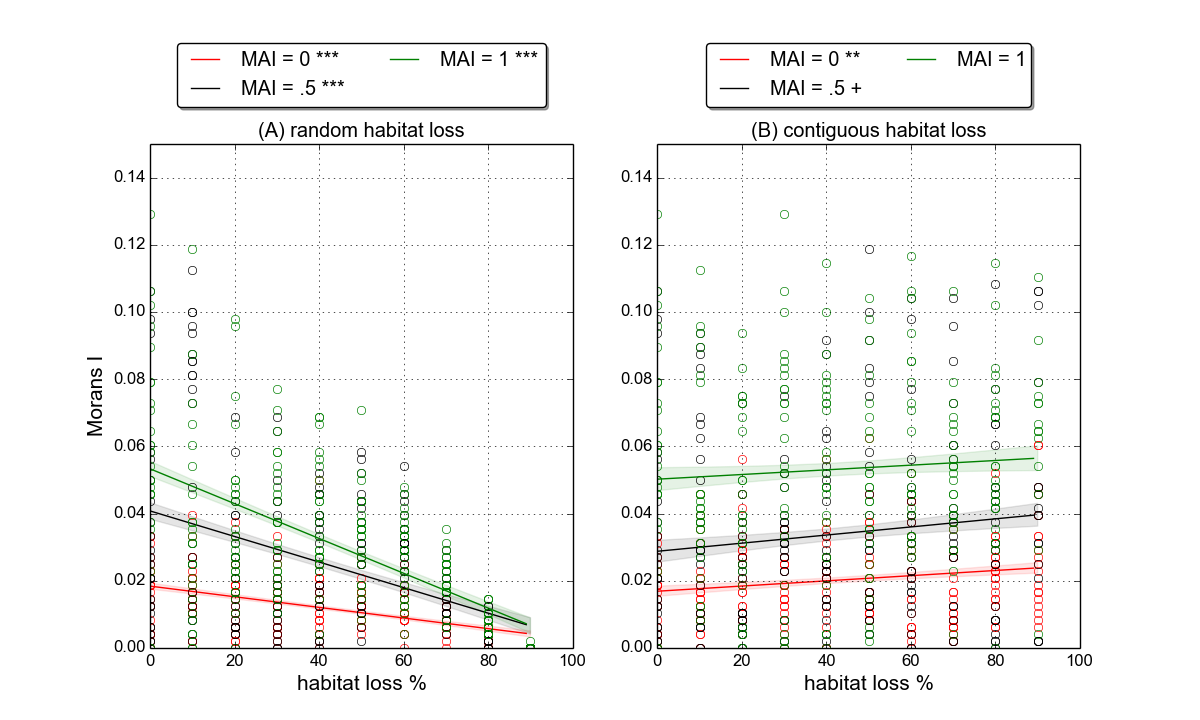
\includegraphics[width=0.9\textwidth]{{{clean_figs/clean_lm_morans_I_3mai}}}
	\caption{\textbf{Moran's I} metric for global aggregation (defined in section \ref{sec:def_spatial_metrics}, averaged over all species. Linear fits and p-value markers as in previous plots (see caption of figure \ref{fig:rel_abun_random}).}
	\label{fig:morans_I}
\end{figure}

\begin{figure}
	\centering
	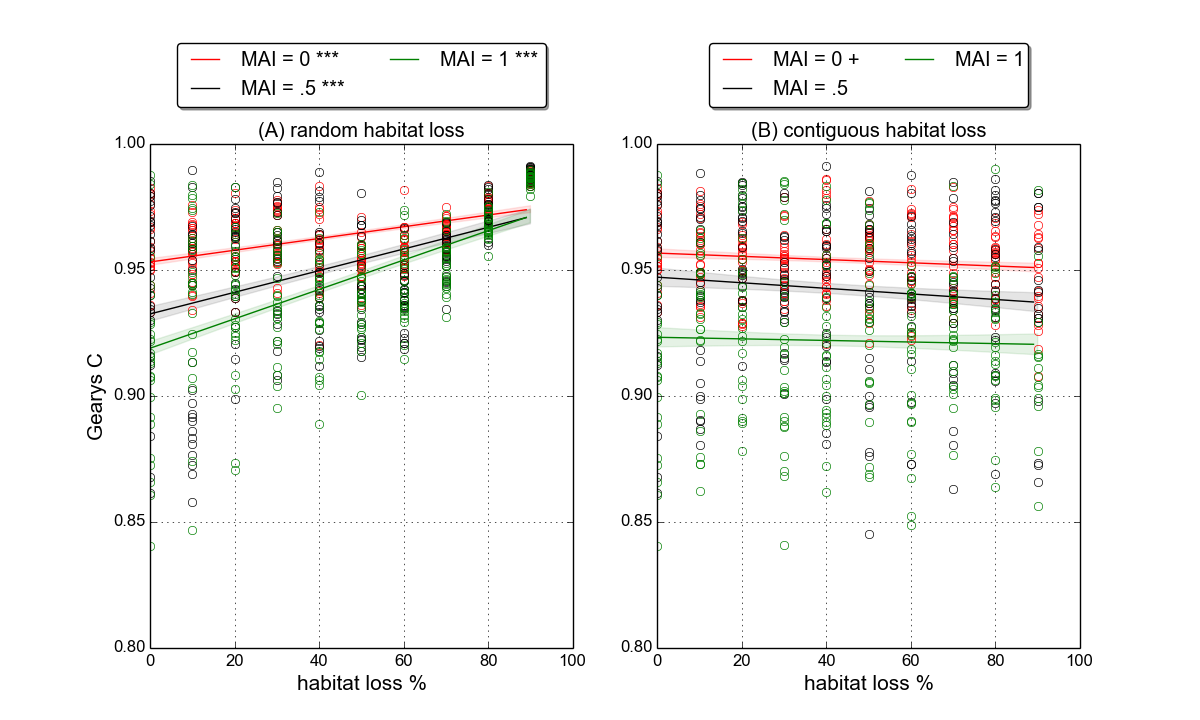
\includegraphics[width=0.9\textwidth]{{{clean_figs/clean_lm_gearys_c_3mai}}}
	\caption{\textbf{Geary's C} metric for local aggregation (defined in section \ref{sec:def_spatial_metrics}, averaged over all species. Linear fits and p-value markers as in previous plots (see caption of figure \ref{fig:rel_abun_random}).}
	\label{fig:gearys_C}
\end{figure}

We observe changes in spatial aggregation under random HL, but not under contiguous HL. Spatial aggregation is measured at the local and global scales using the metrics \emph{Geary's C} and \emph{Moran's I} respectively. Both metrics are bound between 0 and 1. A value of Geary's C close to 0 indicates high locals aggregation, whereas a value of Moran's I close to 1 indicates high global aggregation. Figures \ref{fig:morans_I} and \ref{fig:gearys_C} indicate that, across the board, species are not highly aggregated on average\footnote{What does a random distribution give?}. Also, as reported in \cite{lurgi2015effects}, higher MAI communities are more aggregated than low MAI communities. This is due to differences in the local demographic processes\footnote{Either explain this or refer to paper. Could look at aggregation by functional group. On maximum aggregation}. In response to random HL, species on average become less aggregated in space at both the local and global scales. This is expected because the way in which habitat is destroyed creates a patchy landscape which acts against aggregation. Conversely there is some evidence that contiguous HL leads to a slight increase in aggregation. However the only significant linear trend is in Moran's I at MAI$=0.0$ (figure \ref{fig:morans_I}B). Therefore we conclude that contiguous HL does not create significant and robust changes in aggregation. This may be linked to the reduction in stability, since dynamics become more variable it may be harder to species to form local aggregations in space.

\clearpage
\subsection{Invariability}
\label{sec:res_invariability}

The alternative stability metrics defined in section \ref{sec:def_stability_metrics} are based on \emph{invariability}. These include minimum invariability, population invariability, ecosystem invariability and ecosystem synchrony. Here we demonstrate that the first three of these metrics respond in the same way to HL as the \emph{variability metrics}, giving more weight to the conclusions on stability. The fourth metric, ecosystem synchrony, gives us a new piece of evidence about how the dynamics of the communities change in response to HL. 

Figure \ref{fig:min_inv} shows the response of minimum invariability to HL. We use the natural log-transform of the data, as in section \ref{sec:stability}, because of the apparent exponential nature of the trends in the raw data. From the figure we see that minimum invariability increases in response to random HL, whereas it decreases in response to contiguous HL. The trends are the same for population and ecosystem invariability, and statistically significant at all MAI ratios (results not shown). These changes in invariability are in agreement with the results of the previous section - community dynamics becomes less variable under random HL, and more variable under contiguous HL. The interpretation of these metrics in CITATION lends support to the conclusion that the observed changes in temporal variability are also associated with changes in the stability of the community in a dynamical systems sense\footnote{ More on this, and link to next chapter. Also mention that minimum invariability is dominated by least abundant species.}.

\begin{figure}[b]
	\centering
	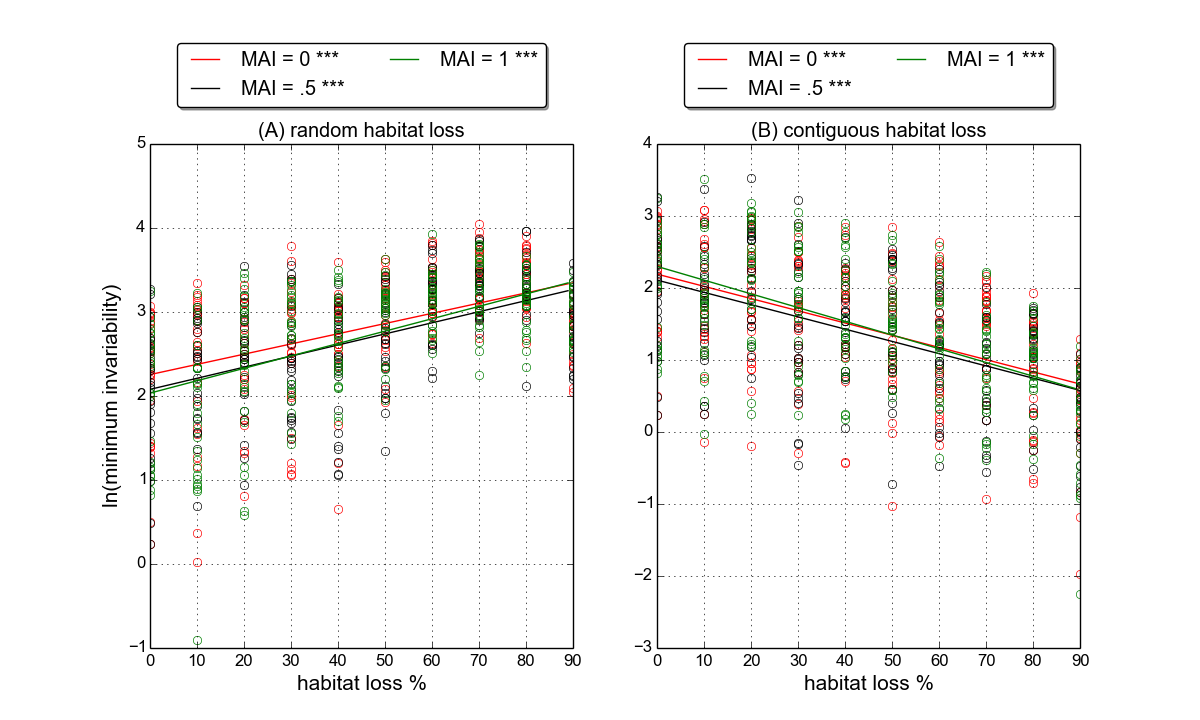
\includegraphics[width=0.9\textwidth]{{{clean_figs/lm_minimum_invariability_3mai}}}
	\caption{\textbf{Minimum invariability} as defined in section \ref{sec:def_stability_metrics}. Linear fits and p-value markers as in previous plots (see caption of figure \ref{fig:rel_abun_random}).}
	\label{fig:min_inv}
\end{figure}

\begin{figure}
	\centering
	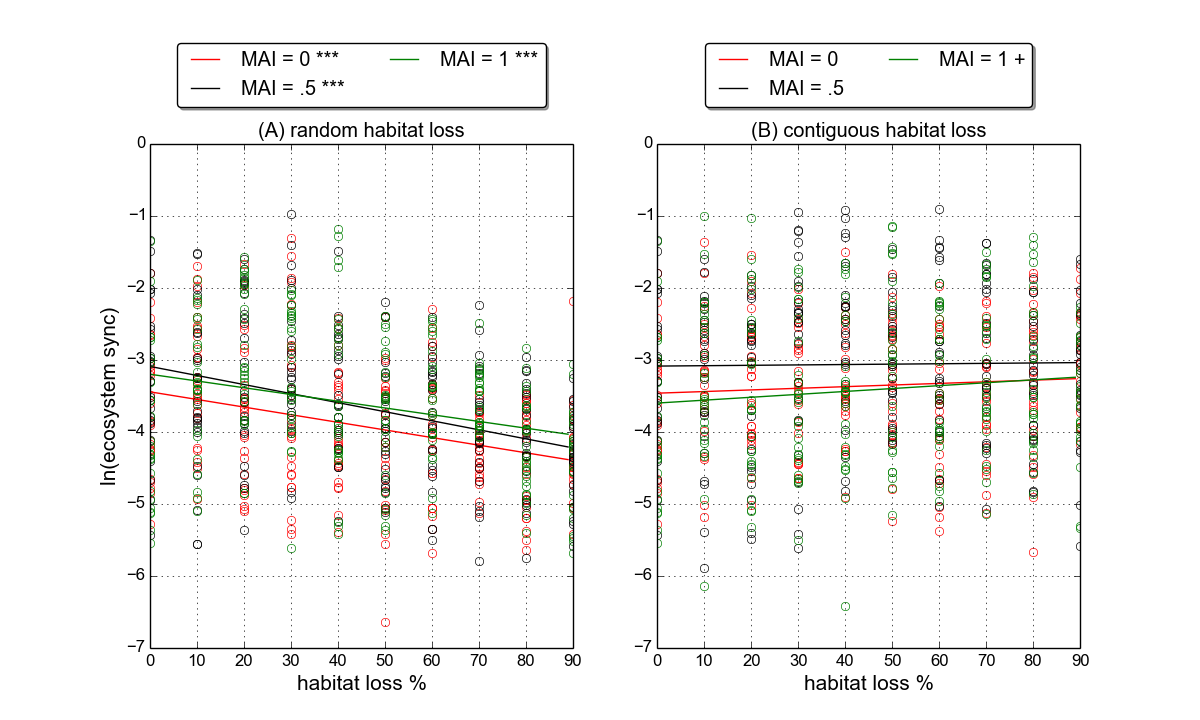
\includegraphics[width=0.9\textwidth]{{{clean_figs/lm_ecosystem_sync_3mai}}}
	\caption{\textbf{Ecosystem synchrony} as defined in section \ref{sec:def_stability_metrics}. Linear fits and p-value markers as in previous plots (see caption of figure \ref{fig:rel_abun_random}).}
	\label{fig:eco_sync}
\end{figure}

Figure \ref{fig:eco_sync} linear fits to the ecosystem level synchrony for the two HL scenarios. In the random case there is a significant decrease in synchrony, whereas in the contiguous case there is no significant change. Also in all cases the synchrony is relatively low. Perfectly synchronised dynamics for all species would give a log-synchrony value of 0. Therefore all communities all well below perfect synchrony. This is expected from trophic dynamics, since it is well known the predator-prey dynamics leads to a phase lag between the population of predator and prey. However it is important to note that trophic dynamics should also lead to some level of synchrony, as species tend to respond in the same to fluctuations in a shared resource or predator. Therefore it may be that the change in synchrony under random HL is a signature that the trophic component of the population dynamics is reduced. This would agree with the observed reduction in interaction strengths shown in figure \ref{fig:strong_fig}.    

\clearpage
\subsection{Synthesis}
\label{sec:res_synthesis}

Here we summarise the results presented so far, and attempt to synthesise them by explaining the main mechanisms driving the observed community responses to HL. Under contiguous HL communities displayed fewer changes than under random HL. \emph{In the contiguous scenario} we saw that the number of individuals,  the frequency of interactions, and to a lesser extent, the number of links, all decreased with HL. However the mean interaction strength and temporal variability increased, representing a reduction in dynamic stability. There were no robust trends in network properties, diversity, evenness, relative abundance by functional group or spatial aggregation, under contiguous HL. \emph{In the random scenario}, as in the contiguous, the number of individuals, the frequency of interactions, and the number of links, all decreased. Unlike the contiguous case, the mean interaction strength and temporal variability decreased, representing an increase in dynamic stability. Under random HL communities became more diverse and more even; displayed a shift in relative abundance towards basal species; and became less aggregated in space. There was also an increase in quantitative vulnerability; a decrease in quantitative generality; and an increase in the interaction diversity of the mutualistic sub-network.

In section \ref{sec:stability} we demonstrated that there is a significant correlation between mean interaction strength and temporal variability. There is good evidence from theoretical population dynamics that strong inter-specific interactions are destabilising [CITATIONS], and there have been some empirical observations of this effect \cite{o2009perturbations}. \emph{Therefore it is reasonable to conclude that the changes in interaction strength are driving the changes in temporal variability}\footnote{MAke this stronger, with explicit reference to LV dynamics.}. In section \ref{sec:res_network_properties} we showed that \emph{the distribution of species abundances can explain the observed changes in quantitative network properties}, or lack thereof. Therefore we are left with two main questions: what is driving the change in interaction strengths? And, what is driving the change in the distribution of species abundances? In what follows we show that the two are closely related.  

In both HL scenarios the total number of individuals and the total number of interactions decreases. However in the random and contiguous scenarios mean interaction strengths decrease and increase respectively. Figures \ref{fig:is3_dist_random} and \ref{fig:is3_dist_contiguous} show that these changes in mean interaction strength are due to the entire distribution of IS3 shifting in opposite directions. Distributions are plotted for MAI$=0.0$ and MAI$=1.0$, showing the same shifts in both cases. We focus on the MAI$=0.0$ case because the pattern is clearer (panel A in these two figures). Under random habitat loss the distribution of IS3 shifts left, towards weaker interactions. The spread also decreases slightly, suggesting less variance in interaction strengths. Under contiguous habitat loss the distribution shifts towards higher interaction strengths, and also becomes much flatter, such that there is a greater spread in interaction strengths. Importantly we see that conclusions based on the mean value of IS3 were not misleading, for example due to a highly skewed distribution. In fact the majority of interactions in a contiguous landscape are stronger than the the majority of interactions in a randomly destroyed landscape, for a given level of HL. However we know, from figure \ref{fig:total_individuals}, that the total number of individuals is similar in either landscape. Since IS3 is calculated by dividing the interaction frequency by the abundance of the two interacting species, it must be the case that interaction frequency is lower for a given number of individuals in a randomly destroyed landscape than a contiguous one. Indeed we saw evidence in figure \ref{fig:total_interactions} that species interact less frequently in the random scenario than the contiguous, despite comparable total numbers of individuals. 

%differential changes in abundance and interaction frequency are responsible for these shifts in the distributions. Put another way, two species with the same number of individuals must interact more frequently in a landscape affected by contiguous HL than one affected by random HL. This is the only way to explain the observed shift in these distribution\footnote{Is this true?}. 

\begin{figure}
	\centering
	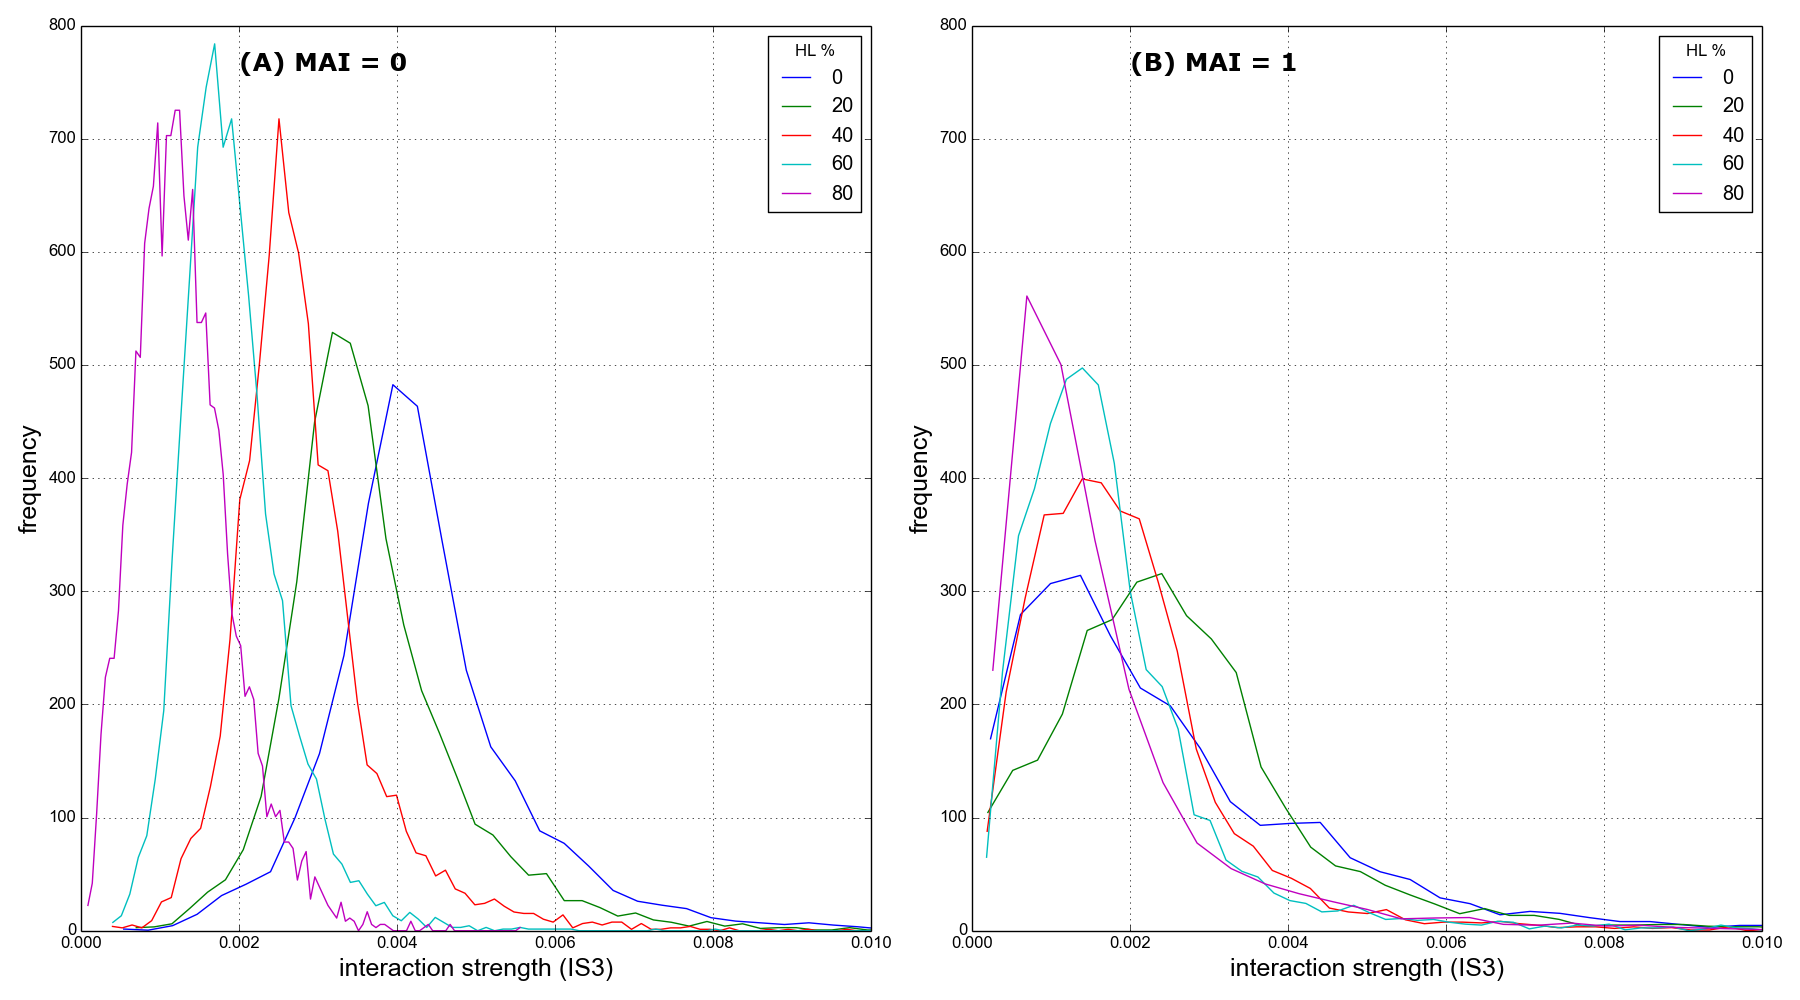
\includegraphics[width=0.9\textwidth]{{{clean_figs/normalised_IS3_dist_random}}}
	\caption{\textbf{Interaction strength distributions (IS3) under random HL.} Panel A: MAI$=0.0$. Panel B: MAI$=1.0$. IS3 values for all interactions in each of 25 replicate simulations at the given MAI and HL value, frequency in 100 bins of equal width. }
	\label{fig:is3_dist_random}
	%% Plotted with chrs_plots_python/scripts/nomralised...py
\end{figure}

\begin{figure}
	\centering
	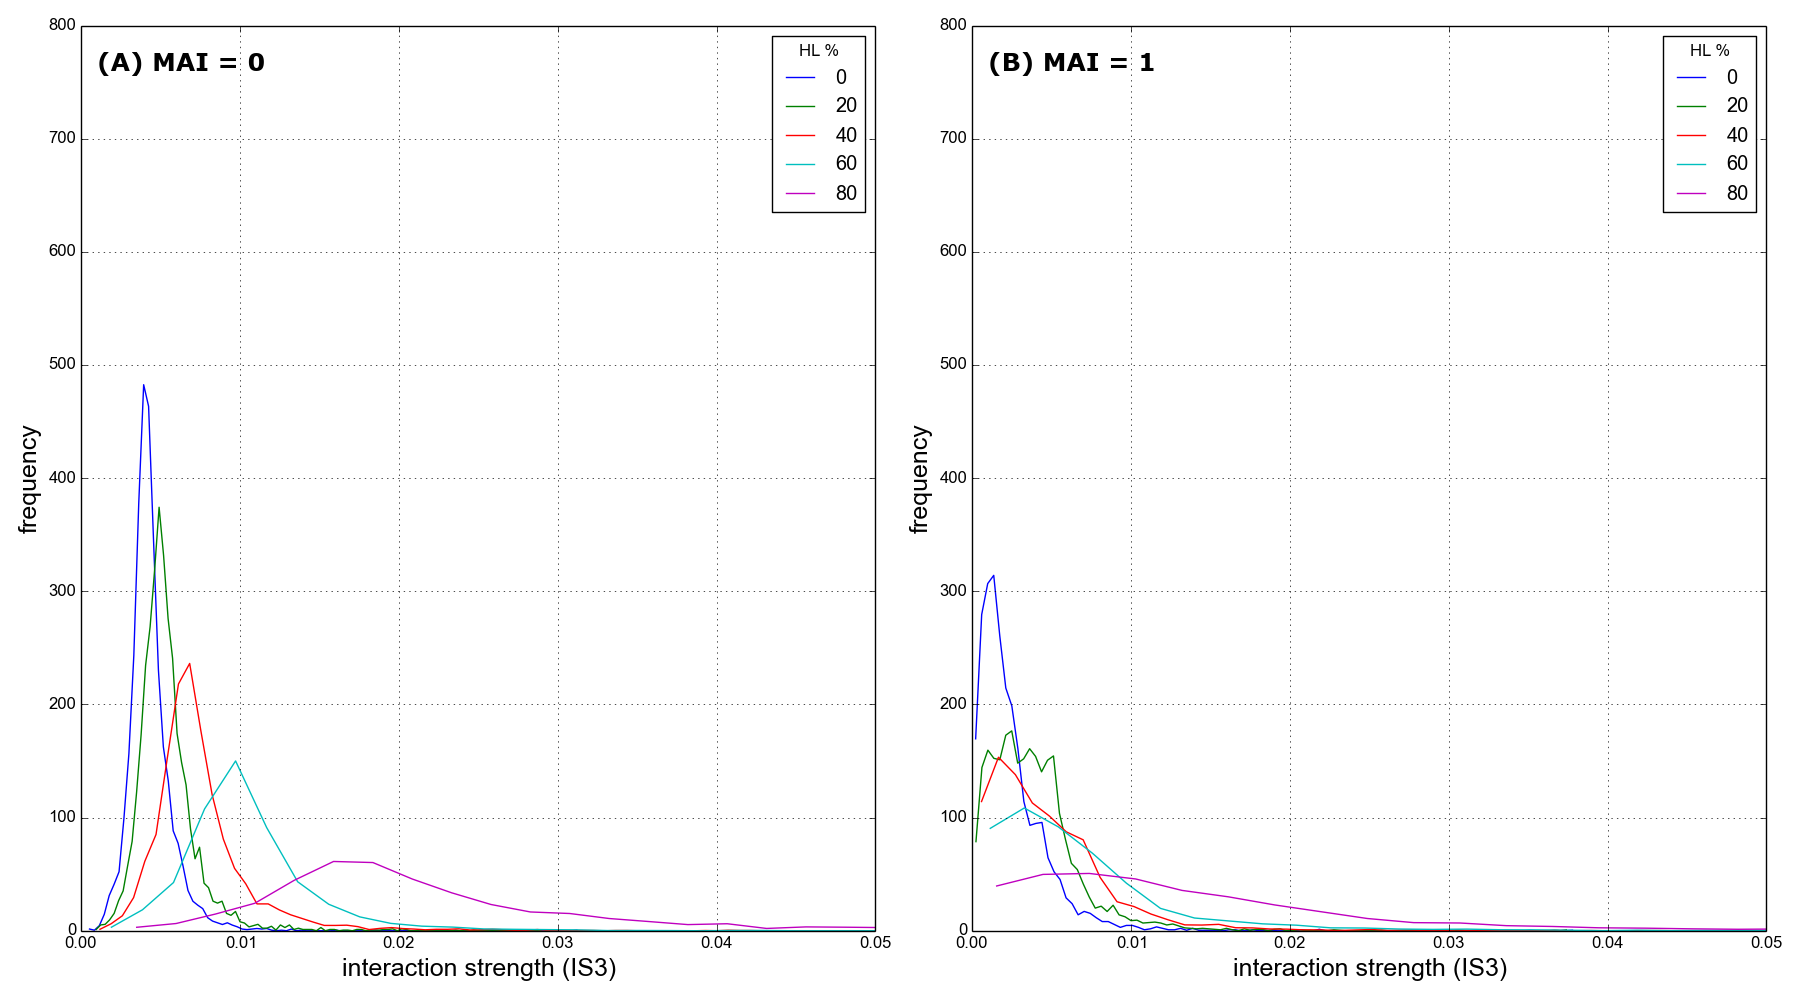
\includegraphics[width=0.9\textwidth]{{{clean_figs/normalised_IS3_dist_contiguous}}}
	\caption{Similar to figure \ref{fig:is3_dist_random}, but for \textbf{contiguous HL.}}
	\label{fig:is3_dist_contiguous}
\end{figure}

Why would species with the same abundance interact more frequently in a contiguous landscape compared to a landscape with random HL? The answer is simply that randomly destroyed cells present a barrier to the motion of individuals. To demonstrate this we conduct a series of simulation experiments, using the following procedure. We place a single individual randomly in a $200 \times 200$ landscape. The  individual moves according to the same rules that the animal individuals follow in the IBM (defined in section \ref{sec:method}), but without the bioenergetic constraints. We record what fraction of the available (i.e. not destroyed) landscape cells the individual visits during 5000 time steps.  The experiment is repeated 100 times for each level of HL, and for both HL scenarios, to obtain the expected range of motion of an individual in each type of landscape. The results are shown in figure \ref{fig:diffusion_example}. Panel A shows an example trajectory of an individual over 5000 iterations in a pristine landscape. Panel B shows the same, but for a landscape at $40\%$ random HL. It is clear that the range of motion is severely restricted by the destroyed cells. Panel C shows that an individual does not experience such barriers to motion in a contiguous landscape, except at the edges of the available habitat. The result is that the percentage of available landscape that an individual can explore during 5000 iterations increases under contiguous HL, but decreases under random HL. This explains the observed changes in interaction strength. If an individual is less mobile it is harder for it to find interaction partners, even if the potential partners are present in the landscape at the same abundance. The converse is true for individuals with increased mobility.

Another consequence of the reduced mobility of individuals is that, \emph{ceteris paribus}, it decreases the probability of intra-specific interactions. These interactions are required for the sexual reproduction of non-basal species - individuals must encounter a member of the same species in space in order to create offspring. Intra-specific interactions are not recorded during the simulations, but the total number of births and total number of immigrants for each species is recorded. In figure \ref{fig:res_proportion_immigrants} we plot the proportion of total births during a simulation that are due to immigration. Here total births includes all new individuals that are created due to immigration, sexual reproduction, mutualistic reproduction, and wind dispersal of plants. From the figure it is clear that immigration is the main source of new individuals - contributing over $50\%$ of new individuals in almost all simulations. However we also see that the relative contribution of immigration is roughly constant under contiguous HL, whereas immigration becomes more important under random HL. We can attribute the differing contribution of immigration, in part, to the changes in mobility illustrated in figure \ref{fig:diffusion_example}. In the random scenario it becomes harder for individuals to find a mate and therefore reproduce, shifting the balance in favour of immigration. In the contiguous case we may expect the opposite - a reduced contribution from immigration due to individual's increased ability to find a mate. It appears that any increase in sexual reproduction due to increased mobility is offset by some other mechanism. One possibility is that the offset is due to increased predator mobility, such that prey species are more likely to be consumed before they can find a mate. This effect may be compounded by the high relative abundance of predator species in the contiguous scenario, even at high levels of HL. The relative abundance and mobility of predators here suggests a strong predation pressure, which is supported by the high inter-specific interaction strengths.

\begin{figure}
	\centering
	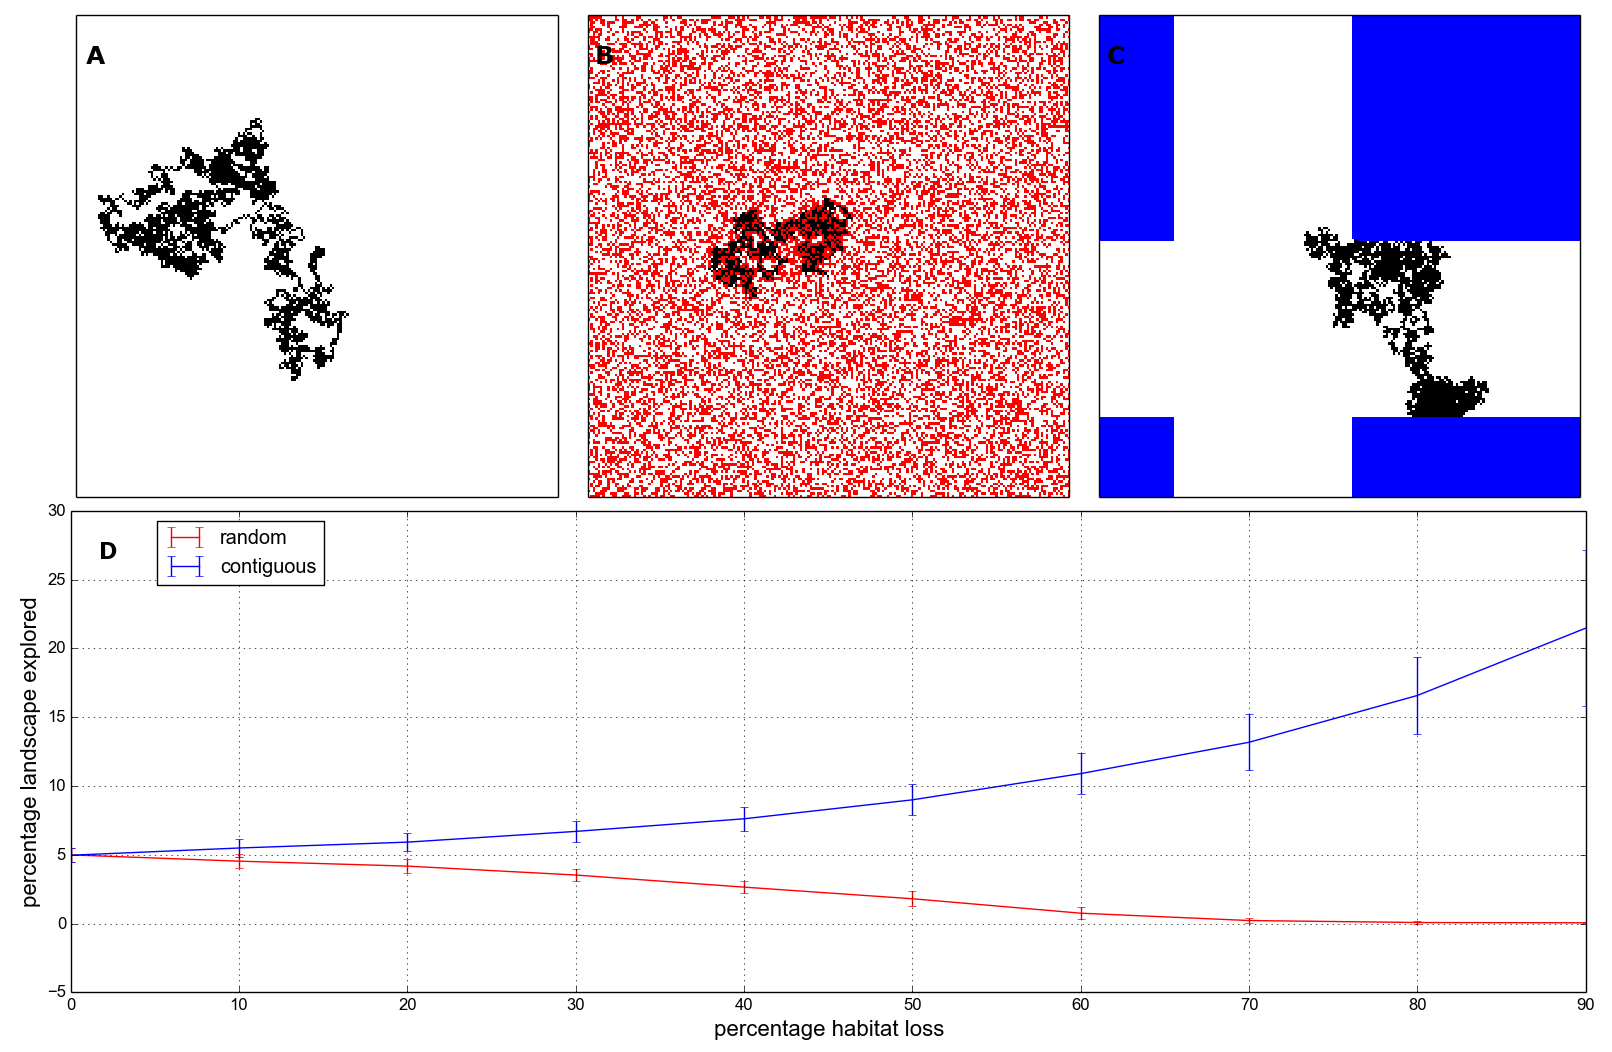
\includegraphics[width=\textwidth]{{{clean_figs/diffusion_example}}}
	\caption{\textbf{An individual\textquotesingle s range of motion} in different habitat conditions. Top row: example trajectory for a single individual over 5000 iterations in (A) pristine landscape; (B) $40\%$ random HL; (C) $40\%$ contiguous HL. Pristine landscape cells shown in white, destroyed cells in  red and blue for random and contiguous destruction respectively. Bottom row (D): Percentage of the pristine landscape cells explored by an individual during 5000 iterations. Solid lines indicate mean over 100 repeat runs; errorbars indicate $\pm 1$ standard deviation.}
	\label{fig:diffusion_example}
\end{figure}

\begin{figure}
	\centering
	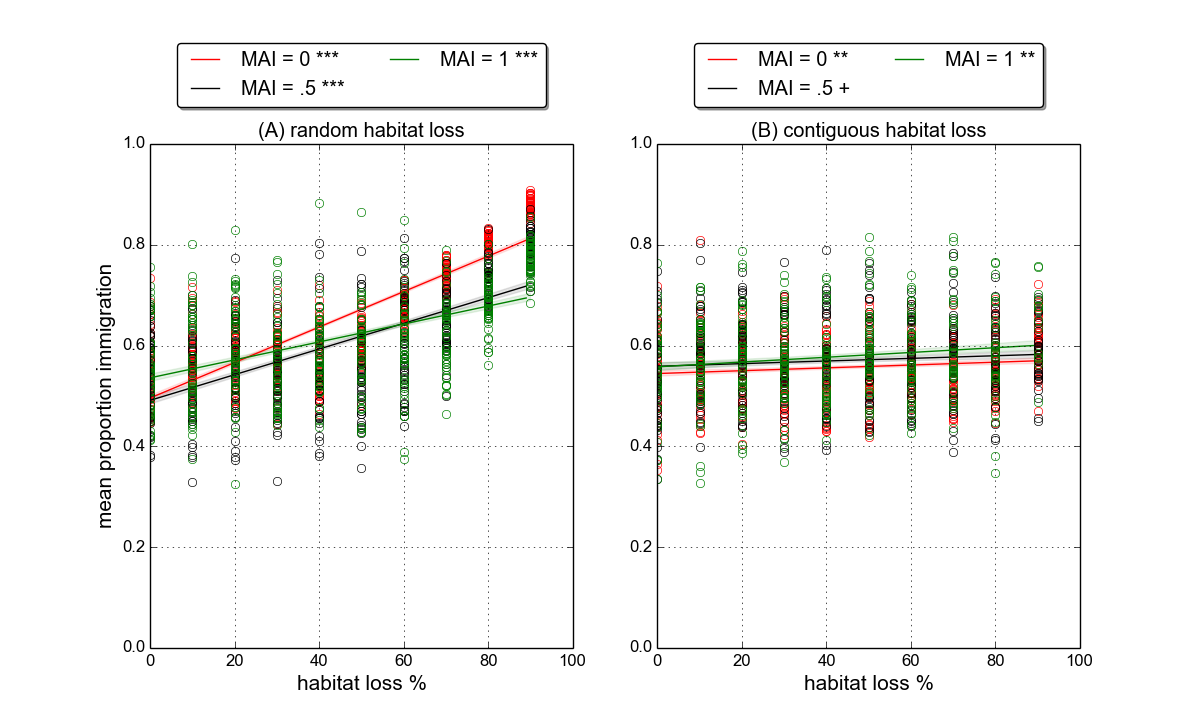
\includegraphics[width=0.9\textwidth]{{{clean_figs/lm_mean_proportion_immigration_3mai}}}
	\caption{\textbf{Number of immigrants} as a fraction of the total number of new individuals created over the course of a simulation. Linear fits and p-value markers as in previous plots (see caption of figure \ref{fig:rel_abun_random}).}
	\label{fig:res_proportion_immigrants}
\end{figure}

We propose that the increased contribution of immigration in the random scenario, but not in the contiguous scenario, explains why some metrics change in one case but not the other. The immigration mechanism is a \emph{levelling influence} on the communities, both spatially and between species. All species are equally likely to immigrate, with no dependence on their abundance or distribution in the landscape. Also all empty cells are equally likely to receive an immigrant at each iteration. Therefore, although there is no spatial preference built into the immigration mechanism, areas of space with a high density of individuals will be locally less likely to receive immigrants than those areas with a low density, simply due to the number of available cells. Therefore immigration, in isolation, acts to make the distribution of individuals more even between species and throughout space. These are both changes that we observe in the random scenario and not the contiguous, and therefore we attribute them, at least in part, to the increased dependence on immigration to supply new individuals.

Another important change, observed in the random but not the contiguous scenario, is the shift in relative abundances of the functional groups. The greatest changes are the increase and decrease in relative abundance of basal and top-predators species respectively. However there is also a decrease in the relative abundance of species in the second trophic level (herbivores and mutualistic-animals). Only omnivore species display no change in relative abundance\footnote{Need to mention difference between high and low mutualism?}. All of these changes in relative abundance can be explained by the change in mobility and its knock on effect on interaction strengths, reproduction and dependence on immigration. The reduction in mobility makes it harder to find prey and results in weaker interaction strengths, as discussed. The result is an overall decrease in predation, meaning that less energy is transferred to the higher trophic levels. The difficulty for animal species to find partners with which to reproduce compounds the effect of reduced energy availability, and this impacts species in the higher trophic levels the most because of cascading effects. Therefore we see a shift in abundance toward basal species, which benefit from the reduced predation pressure and also, in the case of wind dispersed plants, do not require an interaction to reproduce\footnote{This argument does not yet include mutualism.}. Omnivore species benefit most from the increased dependence on immigration than other groups, because this group contains the most species, due to the way that the networks are constructed (see section \ref{sec:interaction_network}). This must explain the constant relative abundance of omnivores\footnote{Also mention that in this chapter predators are omnivorous!}.

It is also worth noting that the increased dependence in immigration is likely the cause of the reduction in ecosystem synchrony observed in section \ref{sec:res_invariability}. The decrease in interaction strengths and increased importance of immigration does indeed reduce the trophic component of the dynamics, in favour of random births due to immigration. We will return to the issue to deterministic versus random dynamics in the nest chapter. 


\clearpage
\section{Discussion}
\label{sec:discussion}

A key feature of these results is that the community response to HL is dependent on the spatial pattern of the perturbation. This has been reported previously in numerous studies [REFS]. Here we have studied the difference between two HL scenarios in more detail, and without focus on extinctions. We have also shown that the main difference between the two scenarios is due to differences in mobility through the landscape, changes in interaction strengths, and differential dependence on immigration from an external source. 

In what follows we will focus on contiguous HL loss. In part this is to simplify the investigation. By only running simulations and presenting results for a single scenario we are able to study the chosen scenario in more detail. The choice of contiguous over random destruction is also justified by realism. In nature habitat tends to be destroyed in a spatially-autocorrelated manner - for example urban development, agriculture and logging all occur in concentrations rather than being distributed totally at random throughout space. Therefore the result of human activity is often a patchy and fragmented landscape [REFS]. The study of our simulated communities under contiguous HL represents the study of communities in single such fragment, with immigration from an external source. In reality we know that such fragments support a lower richness of species, beyond a certain size. In this chapter we saw that a high immigration rate prevented a loss of species richness. In the next chapter we begin to look at how communities respond to changes in the immigration rate.

Also to discuss:
\begin{itemize}
	\item Role of interactions and immigration in maintaining biodiversity and community structure under perturbations.
	
	\item Importance of interaction strengths throughout the thesis: return explicitly in final chapter. 
	
	\item Departures from our results in natural communities: what might be different?
	
	\item Implications for structure-stability debate
	
	\item More explicit discussion of Tylianakis 
	
	\item Why does IS3 change more or less depending on MAI ratio? (referenced to here in text.)
\end{itemize}  

%There it would also be interesting to study the random scenario in more detail, but at this stage we must make decisions to focus the research.

%Another important feature of the results is the importance of interaction strengths. We have shown that stronger interactions lead to increased temporal variability. We have also shown that intra- and inter-specific interactions, and immigration combine to generate community structure (in terms of diversity and the distribution or abundances across species and functional groups). In particular it appears that strong trophic interactions and immigration rates are keys to maintaining biodiversity patterns in the simulated communities.

%The importance of inter-actions will play a an important role throught the thesis. We will return explicitly to study interaction strengths in the final chapter (where we will shown e.g. that higher interaction strengths lead to greater variability).

%The contiguous scenario, which represents a community in a forest fragment...biodiversity is maintained by immigration.

%Close the chapter with..lack of extinctions. However we know that fragments can support fewer species [REFS]. Also we have shown that immigration is the dominant source of new individuals, compared to local demographic processes! What happens when we turn down/off immigration?...  

%\begin{itemize}
%	\item In a real community departures from our model may lead to different results (but also if the same mechanisms are in place we may expect to see something similar), for example:
%	\begin{enumerate}
%		\item In real communities different dispersal and immigration rates for different trophic levels
%		\item Heterogeneous landscape and preferences	
%	\end{enumerate}
%
%
%	\item Immigration being high - want to study lower IR!
%	\item Why definition of extinctions may not be a good one..
%	
%	\item SEM modelling?
%	\item Sensitivity analysis..
%	
%	\item discuss omnivory benefit in random HL case (in fact TP are omnivores here too, but these offset by drop in their predators...?) - in synthesis (that's where it is referred to)
%	
%	\item In quantitative network ecology IS1 is used, but for dynamics and stability IS3 is the key... 
%	
%	\item Refd in text: why does IS3 change less/more based on MAI ratio? (in the random case)
%	
%	\item Importantly these changes occur in the absence of species extinctions, an effect that has been osberved in empir was reported in the empirical finding of Tylianakis \cite{} 
%	
%	\item The results do not suggest that modularity/nestedness are not associated with stability, but rather that stability can change dramatically in different ways without changes in these properties.
%
%\end{itemize}
%
%However the immigration rate is effectively constant across all species (see description of mechanism in section \ref{sec:method}) so that an extinct species may recover by immigrating to a randomly selected lattice cell. The immigration rate (IR) gives the probability that an empty cell receives an immigrant on each iteration. Therefore the default value, IR$=0.005$, would give an expected 200 ($=0.005 \times 200 \times 200$) new immigrants on each iteration, if the landscape were empty\footnote{MOve this discussion to somewhere else} 

%
%\section{OLD STUFF}
%
%
%%Commented out here. No change from previous version.
%
%For both habitat loss scenarios there is no loss of species richness up to $90 \%$ habitat loss. However significant changes are observed in metrics relating to community composition, network properties and stability. In general the qualitative response of these metrics is not governed by MAI ratio i.e. the direction of the trends are the same across MAI ratios, although the extent of the response may vary.
%
%\begin{figure} 
%		\centering      
%		%% ARCEHTYPAL SUBOTTOM CHANGES... (ADD TO PREAMBLE?)
%		\renewcommand{\thesubfigure}{}% no subfigure number
%		\tightsubcaptions % we want tight subcaptions
%		\setlength{\subfloatlabelskip}{0pt}% no space between number and caption
%		
%		\subbottom[]{
%        %\begin{subfigure}[b]{0.5\textwidth}
%                \includegraphics[width=0.45\linewidth]{"random_plots/Total abundance"}}
%%
%        ~
%        \subbottom[]{
%        %\begin{subfigure}[b]{0.5\textwidth}
%                \includegraphics[width=0.45\linewidth]{"contiguous_plots/Total abundance"}}
%        %\end{subfigure}
%
%        \caption{\textbf{Mean total number of individuals} across replicate commmunities decreases with habitat loss, for all MAI ratios. Left: random destruction. Right: contiguous destruction.}\label{fig:total_abundance}
%\end{figure}
%
%Although habitat destruction does not lead to extinctions, it does reduce the total biomass of the communities. This is measured by the total number of individuals of all species remaining at the end of a simulation, which we average across replicate communities. Figure \ref{fig:total_abundance} shows that, although mutualistic communities contain more biomass, the loss of biomass due to habitat destruction is ubiquitous. This is not surprising.
%
%\begin{figure} 
%		\centering      
%		\subbottom[]{
%        %\begin{subfigure}[b]{0.5\textwidth}
%                \includegraphics[width=0.45\textwidth]{"random_plots/mean_cv"}
%        %\end{subfigure}%
%        }
%        ~
%		\subbottom[]{
%        %\begin{subfigure}[b]{0.5\textwidth}
%                \includegraphics[width=0.45\textwidth]{"contiguous_plots/mean_cv"}
%        %\end{subfigure}
%        }
%        \caption{\textbf{Mean CV in total biomass} across replicate commmunities against habitat loss for selected MAI ratios. Left: random destruction leads to an increase in temporal stability, as indicated by a decrease in CV. Right: contiguous destruction drammatically reduces temporal stability.}\label{fig:temporal_stability}
%\end{figure}
%
%How community stability is affected by loss of habitat is of particular interest. Temporal stability is measured by the coefficient of variation (CV) of the total biomass of the system. (This metric is calculated over a number of iterations after the transient dynamics.) A higher CV indicates lower stability, because there are greater fluctuations in the dynamics. We observe that temporal stability is affected differently by the two habitat loss scenarios. As shown in figure \ref{fig:temporal_stability}, random destruction increases temporal stability, whereas contiguous destruction decreases it. What is driving this different response in the dynamics?    
%
%\begin{figure} 
%		\centering      
%		\subbottom[]{
%%        \begin{subfigure}[b]{0.5\textwidth}
%                \includegraphics[width=0.45\textwidth]{"random_plots/IS3"}
%        }%\end{subfigure}%
%        ~
%		\subbottom[]{
%%        \begin{subfigure}[b]{0.5\textwidth}
%                \includegraphics[width=0.45\textwidth]{"contiguous_plots/IS3"}
%        }%\end{subfigure}
%        \caption{\textbf{Interaction strengths:} The sum of the elements of the interaction matrix, averaged over replicate commmunities, for selected MAI ratios. Left: random destruction reduces total interaction strength. Right: contiguous destruction drammatically increases total interaction strength.}\label{fig:IS3}
%\end{figure}
%
%From figure \ref{fig:IS3} it is clear that the response in temporal stability is closely correlated with interaction strengths, as measured by the metric IS3. Random habitat destruction is characterised by a decrease in total interaction strength, whereas contiguous destruction results in a dramatic increase. It is reasonable to assume that these changes in IS3 are causing the different responses in temporal stability. This is supported by the literature, where it is well documented that strong trophic interactions destabilise population dynamics [REFERENCES]. It is not so obvious what affect on dynamics should be expected from an increase in the strength of mutualistic interactions, which are included in this metric. However, figures \ref{fig:temporal_stability} and \ref{fig:IS3} suggest that this is also destabilising.
%
%\begin{figure} 
%		\centering      
%		\subbottom[Random destruction]{
%%        \begin{subfigure}[b]{0.5\textwidth}
%                \includegraphics[width=0.45\textwidth]{"random_plots/interaction_strength_distributions"}
%        }%\end{subfigure}%
%        ~
%		\subbottom[Contiguous destruction]{
%%        \begin{subfigure}[b]{0.5\textwidth}
%                \includegraphics[width=0.45\textwidth]{"contiguous_plots/interaction_strength_distributions"}
%        }%\end{subfigure}
%        \caption{\textbf{IS3 distributions:} The interaction strength distribution shifts leftwards for random habitat loss, and rightwards for contiguous loss. The extent of this shift is mediated by MAI ratio - it is most visibile for MAI$=0$, and least visbile for MAI$=1$.}\label{fig:IS3_distributions}
%\end{figure}
%
%The trends in total interaction strength are due to underlying shifts in the distribution (figure \ref{fig:IS3_distributions}). This is made visible by a shift in the modal peak to lower or higher interaction strengths, for random or contiguous loss respectively. The extent of this shift is mediated by MAI ratio, with greater shifts for lower levels of mutualism.
%
%
%\begin{figure}[ht!]
%		\centering      
%        \includegraphics[width=\textwidth]{"comparison_plots/compare_moransI_mean"}
%        \caption{\textbf{Spatial autocorrelation:} Moran's I is calculated for all species distributions and averaged over the community. These plots show the results averaged over all replicates and over all MAI ratios. Solid lines indicate the mean value, and shaded areas indicate $\pm 1$ standard deviation. This metric suggests that species distributions, on average, become less aggregated in space due to random destruction. Whereas they appear to become more spatially aggregated as a result of contiguous destruction.}\label{fig:morans_i}
%\end{figure}
%
%
%What is causing the different responses of IS3 to the different habitat loss scenarios? Spatial aggregation of species distributions is quantified using Moran's I [REFERENCE]. According to this metric, species distributions become less aggregated in space as a result of random destruction (figure \ref{fig:morans_i}). Whereas they appear to become more aggregated in space under contiguous destruction. If species are more aggregated in space, it may be easier to find an interaction partner. This would benefit predators (and mutualists), potentially leading to stronger de-stabilising trophic interactions. The mean frequency of interactions (figure \ref{fig:IS1}) shows some evidence for this effect. On average there are fewer interactions in communities suffering random habitat destruction, than those with contiguous destruction. However the difference is small, suggesting another mechanism is required to explain the strong responses of IS3 and temporal stability. 
%
%
%It is likely that other changes in network properties and community composition can explain the changes in IS3. The elements of the interaction matrix, used to calculate IS3 are given by \cite{wootton2005measurement, berlow2004interaction}:
%
%\begin{equation}
%\alpha_{ij} = \frac{b_{ij}}{N_i N_j},
%\end{equation} 
%
%where $\alpha_{ij}$ is the effect of species $j$ on species $i$; $b_{ij}$ is the biomass flow from $i$ to $j$ (here measured by the frequency of the interaction, equivalent to IS1) and $N_i$, $N_j$ are the number of individuals belonging to species $i$ and $j$ respectively. Therefore the elements of the interaction matrix are dependent on the relative abundances of the interacting species, as well as the frequency of the interaction. A more detailed analysis of community composition will let us explain to observed trends.    
%
%
%
%
%%This result seems intuitive since and may explain the different responses in IS3. In the case of contiguous loss individuals are contained within a smaller heterogeneous landscape. This effectively reduces the search space for an interaction partner (although the number of potential interaction partners also decreases).  Whereas random loss effectively introduces barriers to dispersal within a landscape of the same total size. 
%
% 
%%\footnote{It should also follow that this effect benefits mutualist species - can we test for this? What does the literature have to say about the effects of stronger mutualistic interactions on temporal stability?}.   
%
%    
%\begin{figure} 
%		\centering      
%        \includegraphics[width=0.6\textwidth]{"comparison_plots/comparing_mean_IS1"}
%        \caption{\textbf{Interaction frequencies:} The metric for interaction strength IS1 averaged over all replicates and all MAI values. This metric is the sum of the elements of the interaction frequency matrix i.e. the total number of interaction occuring within a given period of time. Solid lines indicate the mean value, and shaded areas indicate $\pm 1$ standard deviation. For contiguous destruction interactions are slighty more frequent, on average, than for random destruction.}\label{fig:IS1}
%\end{figure}
%
%\newpage
%\section{More preliminary results}
%\label{sec:more_results}
%
%By averaging results over MAI ratios we are able to effectively obtain more replicate communities. When doing this certain metrics appear to display trends in response to habitat loss that are not clearly visible without this averaging. We perhaps need to justify this approach, and to fit statistical models to quantify the significance of the trends in certain metrics. 
%
%
%\begin{figure}[b!]
%		\centering      
%        \includegraphics[width=\textwidth]{"comparison_plots/compare_shannoneq_mean"}
%        \caption{\textbf{Shannon evenness:} average over MAI ratios and replicate communities. Under random habitat destruction communities on average become more even. Under contiguous destruction there is no change.}\label{fig:shannon_eq}
%\end{figure}
%
%\begin{figure}
%		\centering      
%        \includegraphics[width=\textwidth]{"comparison_plots/compare_h2_mean"}
%        \caption{\textbf{Specialisation:} H2' is a metric that qunatifies the degree of specialisation of interactions in the mutualistic sub-network. Mutualists appear to become less specialised under random destruction, and more specialised under contiguous. (This appears to disagree with previous plots of H2, but I can't see why - the numbers used are taken from output\_network.csv, column titled H2.) }\label{fig:h2}
%\end{figure}
%
%\begin{figure}[p] 
%		\centering      
%        \includegraphics[width=\textwidth]{"random_plots/RADs_mut0"}
%        \caption{\textbf{RADs for Random habitat loss:} Rank abundance distributions for MAI$=0$, three replicate communities shown for slelected levels of habitat loss (0,50,90). In the case of random destruction we expect the communities to become more even on average, based on Shannon\_Eq metric, (figure \ref{fig:shannon_eq})}\label{fig:RADS_random}
%\end{figure}
%
%
%\begin{figure}[p] 
%		\centering      
%        \includegraphics[width=\textwidth]{"contiguous_plots/RADS_mut0"}
%        \caption{\textbf{RADs for Contiguous habitat loss:} Rank abundance distributions for MAI$=0$, three replicate communities shown for slelected levels of habitat loss (0,50,90). In the case of contiguous destruction we expect no trend in evenness on average, based on Shannon\_Eq metric, (figure \ref{fig:shannon_eq})}\label{fig:RADS_contiguous}
%\end{figure}
%
%
%\section{Further development and work to do}
%
%\subsection{Work to do}
%
%\begin{itemize}
%	\item Write introduction
%	\item Write up ecological metrics
%	\item Amend figure captions
%	\item Plot example networks
%	\item Plot dynamics
%	\item Analyse dynamics (transience, steady-state)
%	\item Fix conflict in trophic level results
%	\item Analyse ecological metrics by trophic level (basal, intermmediate, top)
%	\item Understanding IS3 response: plot $IS1/N^2$, look at individual runs
%	\item Compare movement of species to diffusion coefficient in porous medium
%	\item Plot RADS with species coloured accroding to trophic level.
%\end{itemize}
%
%\subsection{Further development}
%
%\begin{itemize}
%	\item Run simulations with lower immigration
%	\item Well mixed approximation. Simplified model for analysys
%	\item Can we calculate robustness from network, and test this against what extinctions we get? (With lower immigration)
%\end{itemize}
